

\chapter{Àlgebra lineal}\label{algebra}
Quan vaig començar a buscar informació sobre computació quàntica, vaig ràpidament vaig adonarme'n que necessitava més coneixements matemàtics, com que no entenia gairebé res dels llibres sobre computació quàntica. Durant aquell temps em van captar l'atenció una sèrie de vídeos sobre àlgebra lineal, que és justament la branca de les matemàtiques sobre la qual es basa la computació quàntica. Aquests vídeos són les lliçons que dona el professor Gilbert Strang a l'Institut Tecnològic de Massachusetts (MIT en anglès) \cite{LA_OCW_strang, LA2_OCW_strang}. Una vegada havia vist gairebé tots els vídeos, ja tenia bastants conceptes apresos.

Aquelles lliçons em van ajudar a entendre les matemàtiques de \textit{Quantum Computation and Quantum Information} \cite{QCandQI} i \textit{Quantum Computing: A Gentle Introduction} \cite{QC_intro}. A poc a poc, vaig anar aprenent els fonaments matemàtics de la computació quàntica i mecànica quàntica.

En aquesta secció explicaré els conceptes bàsics de l'àlgebra lineal amb la finalitat de situar els antecedents teòrics d'aquesta recerca. 

\section{Vectors i espais vectorials}
Els objectes fonamentals de l'àlgebra lineal són els espais vectorials. Un espai vectorial és el conjunt de tots els vectors amb les mateixes dimensions i amb certes propietats en comú. Per exemple $\mathbb{R}^{3}$ seria l'espai vectorial de tots els vectors de 3 dimensions els quals normalment s'utilitzen per representar punts en un espai tridimensional. En computació quàntica es fan servir uns espais vectorials anomenats espais de Hilbert, que són aquells en els que hi ha definit un producte interior \cite{QCandQI:GramSchmidt}. En els espais de Hilbert es defineixen un conjunt d'operacions amb certes propietats, les quals explicaré a continuació. S'ha de tenir en compte que els espais de Hilbert són molt més complicats que el que es representa en aquest treball. En endavant, quan mencioni espai vectorial, em referiré a un espai de Hilbert.

Els espais vectorials estan definits per les seves bases, i.e. un conjunt de vectors independents $B = \{\ket{v_1}, \cdots, \ket{v_n}\}$. Posat d'una altra manera: el conjunt $B$ és una base pel l'espai $V$, si cada vector $\ket{v}$ en l'espai es pot escriure com $\ket{v} = \sum_i a_i \ket{v_i}$ per $\ket{v_i} \in B$.

La notació estàndard per l'àlgebra lineal en mecànica quàntica és la notació de Dirac, en la qual es representa un vector com $ \ket{\psi} $ (on $\psi$ és la etiqueta del vector). Un vector $ \ket{\psi} $ amb $n$ dimensions també pot ser representat com una matriu columna que té la forma: 
$$
\ket{\psi} = 
\begin{bmatrix}
	z_{1} \\
	z_{2} \\
	\vdots \\
	z_{n-1} \\
	z_{n}
\end{bmatrix}
$$

Pels seus elements $\{z_{1}, z_{2}, \cdots , z_{n-1}, z_{n}\} \in \mathbb{C}$ . Els vectors escrits com $\ket{\psi}$ s'anomenen \textit{ket}.

En els espais de Hilbert es defineix una addició de vectors\footnote{Els vectors d'aquesta definició tenen els seus elements representats per la seva etiqueta i un subíndex e.g. el vector $\ket{\psi}$ té un element qualsevol $\psi_{i}$ i el seu primer element es $\psi_{1}$. Aquesta notació es seguirà utilitzant al llarg del treball.}:
$$
\ket{\psi} + \ket{\varphi} = \begin{bmatrix} \psi_{1} \\ \vdots \\ \psi_{n} \end{bmatrix} +
\begin{bmatrix} \varphi_{1} \\ \vdots \\ \varphi_{n} \end{bmatrix} = 
\begin{bmatrix} \varphi_{1} + \psi_{1} \\ \vdots \\ \varphi_{n} + \psi_{n} \end{bmatrix}
$$

I una multiplicació escalar:
$$
  z\ket{\psi} = z\begin{bmatrix} \psi_{1} \\ \vdots \\ \psi_{n} \end{bmatrix} = \begin{bmatrix} z \psi_{1} \\ \vdots \\ z \psi_{n} \end{bmatrix}
$$
Per a un escalar $z$ i dos vectors $\ket{\psi}$ i $\ket{\varphi}$.

A més a més, hi ha definit un conjugat complex: Per $z=a +bi$, el seu conjugat $z^*$ és igual a $a-bi$. 

Aquesta noció es pot ampliar també a les matrius:
$$
\ket{\psi}^{*} = 
	\begin{bmatrix} \psi_{1} \\ \vdots \\ \psi_{n} \end{bmatrix}^* = \begin{bmatrix} \psi_{1}^* \\ \vdots \\ \psi_{n}^* \end{bmatrix}
$$
$$
A^{*} = 
	\begin{bmatrix} 
	a_{11} & \cdots & a_{1n}\\ 
	\vdots & \ddots & \vdots \\ 
	a_{m1} & \cdots & a_{mn}
\end{bmatrix}^* 
= \begin{bmatrix} 
	a_{11}^* & \dots & a_{1n}^*\\ 
	\vdots & \ddots & \vdots \\ 
	a_{m1}^* & \cdots & a_{mn}^*
\end{bmatrix}
$$
Amb $\ket{\psi}$ sent un vector de dimensions $n$, i $A$ sent una matriu de dimensions $m \times n$.

Un altre concepte important és la transposada, representada pel superíndex $T$ que «rota» un vector o una matriu. Un vector columna amb una dimensió $n\times 1$ es transforma a un vector fila amb una dimensió $1\times n$\footnote{En realitat els vectors columna son matrius amb dimensió $n,1\,$, però he estat ometent el 1. Quan em refereixo a les dimensions d'un vector qualsevol, només diré un nombre, no obstant això, especificaré si és un vector columna o un vector fila.}:
$$
\ket{\psi}^{T} = 
	\begin{bmatrix} \psi_{1} \\ \vdots \\ \psi_{n} \end{bmatrix}^T = \begin{bmatrix} \psi_{1} & \dots & \psi_{n} \end{bmatrix}
$$

El mateix és cert per les matrius, una matriu $m\times n$ transposada es converteix en una matriu $n \times m$:
$$
A^T = \begin{bmatrix}
	 2 & 3 \\
	 6 & 4 \\
	 2 & 5 
\end{bmatrix}^T = \begin{bmatrix}
 2 & 6 & 2 \\
 3 & 4 & 5
\end{bmatrix}
$$

La composició d'un conjugat complex i la transposada s'anomena el conjugat Hermitià, la seva notació és una $\dagger$ superindexada. Per un vector $\ket{\psi}$ el seu conjugat Hermitià $\ket{\psi}^\dagger$ és:
$$
\ket{\psi}^\dagger = (\ket{\psi}^*)^T =  \begin{bmatrix} \psi_{1}^* & \cdots & \psi_{n}^* \end{bmatrix} = \bra{\psi}
$$
El conjugat Hermitià compleix que $\ket{\psi}^\dagger = \bra{\psi}$ i $\bra{\psi}^\dagger = \ket{\psi}$.

El conjugat Hermitià d'un vector columna $\ket{\psi}$ s'anomena \textit{bra} o vector dual. En la notació de Dirac un vector dual s'escriu com $\bra{\psi}$.

\section{Aplicacions lineals}
Per poder operar amb vectors i fer operacions amb ells, s'utilitzen les matrius, que també son anomenades aplicacions lineal o transformacions lineals; noms que descriuen millor com funcionen aquests objectes. La definició formal d'una aplicació lineal pot ser bastant complicada, per aquesta raó, faré servir termes més informals en aquesta secció. 

Bàsicament, una aplicació lineal transforma un vector en un altre vector, que poden o no ser d'espais diferents \cite{LR_done_right:linear_map}. Millor dit: per un vector $\ket{v}$ en un espai $V$ i un vector $\ket{w}$ en un espai $W$, una aplicació lineal $A$ entre els vectors, fa l'acció:
$$
A \ket{v} = \ket{w}
$$
En altres paraules, aquesta aplicació transforma un element del espai vectorial $V$ en un element de l'espai vectorial $W$.
Les aplicacions lineals han de complir les següents propietats:
\begin{enumerate}
	\item Addició de vectors: \\
	Donats els vectors $\ket{\psi}$ i $\ket{\varphi}$ en un mateix espai vectorial, i una aplicació lineal $A$:
	$$ A(\ket{\psi} + \ket{\varphi}) = A\ket{\psi} + A\ket{\varphi}$$ 
	\item Producte escalar:\\
	Donats els vectors $\ket{\psi}$, l'escalar $z$ i la transformació lineal $A$, és cert que:
	$$ A(z\ket{\psi}) = z A \ket{\psi}$$
\end{enumerate}

Aquestes afirmacions han de ser certes per tots els vectors i tots els escalars en els espais on les aplicacions actuen. Cal notar que una aplicació lineal no té perquè ser una matriu necessàriament, per exemple, les derivades i les integrals son aplicacions lineals. Això es pot provar fàcilment al veure que compleixen els criteris especificats posteriorment. Tanmateix, les derivades i les integrals usualment no s'apliquen a vectors, sinó a les funcions, però és possible aplicar-les a vectors.

Les matrius serien la representació matricial de les aplicacions lineals \cite{LR_done_right:matrix}.

\subsection{Tipus d'aplicacions lineals}
En la secció actual, exposaré els tipus bàsics d'aplicacions lineals que són indispensables en la teoria presentada en aquest capítol i la resta del treball.

\begin{enumerate}
	\item \textbf{Operador zero} \\
	Qualsevol espai vectorial té un vector zero expressat en notació de Dirac com a $0$, pel fet que $\ket{0}$ és un altre concepte totalment diferent en CQ i IQ\footnote{Computació Quàntica i Informació Quàntica.}. També es pot escriure com a $0$. Es aquell vector que per qualsevol vector $\ket{\psi}$ i qualsevol escalar $z$, es compleix que: 
	\begin{enumerate}
		\item És l'element neutre: $\ket{\psi} + 0 = \ket{\psi} $
		\item I l'element nul pel producte escalar: $z0 = 0$. 
	\end{enumerate}
	
	
	\item \textbf{Matriu inversa} \\
	Una matriu quadrada\footnote{Una matriu quadrada és una matriu amb dimensions $n\times n$, on $n \in \mathbb{N}$.} $A$ és invertible si existeix una matriu $A^{-1}$ de manera que $AA^{-1}=A^{-1}A = I$, on $A^{-1}$ seria la matriu inversa de $A$. La manera més ràpida de saber si una matriu és invertible és verificant si el seu determinant no és zero.

	\item \textbf{Matriu Identitat} \\
	Per a qualsevol espai vectorial $V$ existeix una matriu $I$ que és definida a partir de $I\ket{\psi} = \ket{\psi}$. Aquesta matriu no fa cap canvi als vectors als quals opera, ni tampoc a les matrius amb les quals es multiplica.
	
	\item \textbf{Matrius Hermitianes} \\
	Una matriu Hermitiana compleix que: 
	$$
	\bra{\psi} (A \ket{\varphi}) = (A^\dagger\bra{\psi})\ket{\varphi}
	$$
	On $\ket{\psi}$ i $\ket{\varphi}$, són dos vectors de l'espai en el qual actua $A$. Aquestes matrius o operadors en mecànica quàntica són molt importants, ja que són els observables d'un sistema quàntic. Per exemple l'operador del moviment lineal d'un electró és un operador hermitià. 
	
	\item \textbf{Matriu Unitària} \\
	Una matriu unitària és qualsevol matriu que no altera la norma\footnote{El concepte generalitzat de la longitud d'un vector. Usualment, parlaré de la norma $\ell_2$, esmentada com $\norm{\cdot}_2$, i definida com a $\norm{\ket{\psi}} = \sqrt{\psi^2_1 + \cdots + \psi^2_n}$.} o longitud dels vectors als quals és aplicada, per tant, una matriu és unitària si $A^\dagger A = I$
	Per convertir qualsevol matriu en unitària, es divideixen els seus components entre la norma de la mateixa matriu.
	
\end{enumerate}

\section{Producte interior i producte exterior}

\subsection{Producte interior}
Un vector dual $\bra{a}$ i un vector $\ket{b}$ combinats formen el producte interior $\bra{\psi}\ket{\varphi}$, el qual efectua una operació que agafa els dos vectors com a input i produeix un nombre complex com a output \cite{QCandQI:inner}:
$$
\bra{a}\ket{b} = a_1 b_1 + a_2 b_2 + \cdots + a_{n-1} b_{n-1} + a_n b_n = z
$$
Amb $z, a_i, b_i \in \mathbb{C}$. Cal notar que els vectors $\ket{a}$ i $\ket{b}$ han de tenir la mateixa mida. 

Aquest producte per dos vectors en $\mathbb{R}^2$ també es pot escriure com a:
\begin{equation}
	\bra{a}\ket{b} = \norm{\ket{a}}_2  \norm{\ket{b}}_2 \cos \theta 
	\label{eq:dot_product}
\end{equation}


Amb $\norm{\cdot}_2$ sent la norma $\ell^2$ i $\theta$ sent l'angle entre els vectors $\ket{a}$ i $\ket{b}$. Com he dit l'equació \eqref{eq:dot_product} és equivalent al producte interior. No obstant això, segons el que he vist aquesta equació no es usada àmpliament, ja que interpretar $\theta$ com un angle entre vectors de dimensions altes no té molt de sentit. 

Usualment, aquest producte es presentat en la seva interpretació geomètrica\footnote{Els detalls exactes de la interpretació geomètrica es troben fora del domini d'aquest treball, malgrat que m'agradaria molt parlar sobre el tema.} com el producte entre un vector fila i un vector columna:
$$
\bra{a}\ket{b} = \begin{bmatrix}a_1^{*}  \cdots  a_n^{*} \end{bmatrix} \begin{bmatrix} b_{1} \\ \vdots \\ b_{n} \end{bmatrix}
$$

Ja he definit la norma $\ell_2$ com l'arrel quadrada de la suma dels elements d'un vector al quadrat:
$$
\norm{\ket{a}}_2 = \sqrt{\sum_{i} \abs{a_{i}}^2}
$$
Tanmateix, la definició més comuna es basa en el producte interior. Com es pot veure el producte interior d'un vector per ell mateix és la suma dels seus components al quadrat:
$$
\bra{a}\ket{a} = a_1 a_1 + \cdots + a_n a_n = a_1^2 + \cdots +  a_n^2 \\= \sum_{i} \abs{a_i}^2
$$
Per tant, la norma pot ser definida com l'arrel quadrada del producte interior d'un vector \cite{LR_done_right:norm}:
\begin{equation}
\norm{\ket{a}}_2 = \sqrt{\bra{a}\ket{a}}
\label{eq:norm}
\end{equation}
Quan la norma és aplicada a un vector bidimensional, es pot veure que és el mateix que la longitud Euclidiana d'aquell vector, això és perquè realment són els mateixos conceptes. Tot i això, la norma és el concepte de longitud però generalitzat a vectors de dimensions altes.

Segons el que he vist, algunes propietats de la longitud d'un vector bidimensional no es mantenen amb la norma d'un vector que té més de 2 dimensions. En altres paraules, la norma es comporta en certes maneres com la distancia des de l'origen (que és la definició de la longitud), però són exactament el mateix. A més d'això, hi ha diferents tipus de normes que s'utilitzen en diversos escenaris. Aquesta és la raó per la qual em refereixo a la norma; com la norma $\ell^2$. A aquesta norma també se li diu norma Euclidiana \cite{wolfram:2norm}.

\subsubsection{Propietats del producte interior}
Les propietats bàsiques del producte interior són les següents \cite{QCandQI:intro}:
\begin{enumerate}
	\item És lineal en el segon argument $\bra{a}(z_{1}\ket{b}+z_{2}\ket{c}) = z_{1}\bra{a}\ket{b} + z_{2}\bra{a}\ket{c}$
	\item $\bra{a}\ket{b} = (\bra{b}\ket{a})^*$
	\item $\bra{a}\ket{a}$ és no negatiu i real, excepte en el cas de $\bra{a}\ket{a} = 0 \iff \ket{a} = 0$
\end{enumerate}

 
\subsection{Vectors ortonormals i ortogonals}
A partir del concepte de norma sorgeixen els conceptes d'un parell de vectors ortonormals i un parell de vectors ortogonals.
Mirant l'equació \eqref{eq:norm}, podem veure que si el producte interior del vector és 1, la norma del mateix vector també és 1. Un vector que té norma 1, és un vector unitari.

Dos vectors diferents de zero són ortogonals si el seu producte interior és zero. Si aquests vectors són bidimensionals, a partir de l'equació \eqref{eq:dot_product} podem veure que el cosinus de l'angle que fan entre ells és zero, són perpendiculars entre ells:
\begin{multline*}
	 \text{Per }\ket{a} \text{i} \ket{b}\neq 0 : \\
	\text{Si }\bra{a}\ket{b} = 0 \text{ tenim que: } \norm{\ket{a}}_2 \cdot \norm{\ket{b}}_2 \cos \theta = 0 \\
	 \text{Perquè $\ket{a}$ i $\ket{b}$ no són zero, les seves normes tampoc ho són.} \\
	 \text{Per tant el terme que falta } \cos\theta \text{ ha de ser igual a zero.} \\
	 \text{D'aquesta manera, l'angle $\theta$ ha de ser } \frac{\pi}{2}. \\
\end{multline*}
No obstant això, pensar que la perpendicularitat i l'ortogonalitat són els mateixos conceptes és un error, això només és veritat pels vectors bidimensionals. Perquè com en el cas de la norma i la longitud, l'ortogonalitat és el concepte de perpendicularitat però generalitzat \cite{LR_done_right:norm}.

Quan barregem els conceptes de vector unitari i vectors ortogonals arribem a l'ortonormalitat \cite{QCandQI:GramSchmidt}. Un parell de vectors que no són zero, són ortonormals quan els dos vectors són unitaris i també són ortogonals entre ells:

$$
\ket{a} \text{ i } \ket{b} \text{ són ortonormals si:} \left\{
	\begin{array}{ll}
		\bra{a}\ket{b} = 0 \\
		\bra{a}\ket{a} = 1 \\
		\bra{b}\ket{b} = 1 \\
	\end{array}
\right.
$$
Els vectors ortonormals són importants. Són àmpliament utilitzats tant en computació quàntica com en mecànica quàntica perquè serveixen per crear bases vectorials que resulten molt útils.

Una altra cosa que remarcar és que al dir un parell de vectors, aquest parell també pot ser un conjunt de vectors. Si un conjunt està compost de vectors unitaris, i aquests són ortogonals entre ells, és un conjunt de vectors ortonormals.
El conjunt de vectors $ B = \{\ket{\beta_1}, \ket{\beta_2}, ..., \ket{\beta_{n-1}} \ket{\beta_n}\} $ és ortonormal si $\bra{\beta_i}\ket{\beta_j} = \delta_{ij}  \forall i, j$ \cite{QCandQI:GramSchmidt} on $\delta_{ij}$ és el Kronecker delta, definit com:
$$
\delta_{ij} =
\begin{cases}
	1 &\text{si } i=j\\
	0 &\text{si } i\neq j
\end{cases}
$$

\subsection{Producte exterior}
El producte exterior és una funció (expressada com $\ket{a}\bra{b}$, amb $\ket{a}$ i $\ket{b}$ sent vectors) que agafa dos vectors i produeix un operador lineal com output. Al contrari que el producte interior, no hi ha un producte equiparable en les matemàtiques ensenyades a l'institut, i és una mica difícil d'entendre perquè agafa dos vectors que poden ser d'un espai diferent com input. És definit com:

Pels vectors $\ket{v}$ i $\ket{v'}$ amb dimensions $m$ i el vector $\ket{w}$ de dimensions $n$. El producte exterior és l'aplicació lineal $A$ de dimensions $m \times n$ en l'espai $\mathrm{Mat}_{m\times n}$:
$$
\ket{v}\bra{w} = A \text{ amb } A\in \mathrm{Mat}_{m\times n} .
$$ 
%In other words, that takes a vector from $\mathbb{C}_i$ to $\mathbb{C}_j$. 
Amb la seva acció definida per \cite{QCandQI:inner}: 
\begin{equation}
	(\ket{w}\bra{v})\ket{v'} \equiv \ket{w}\bra{v}\ket{v'} = \bra{v}\ket{v'}\ket{w}
	\label{eq:outer_def}
\end{equation}

A partir de l'equació \eqref{eq:outer_def} la utilitat i significat del producte són bastant complicats d'entendre, per tant, exposaré la manera de computar-lo per clarificar com funciona. Per dos vectors $\ket{a}$ i $\ket{b}$ de dimensions $m$ i $n$ respectivament, el seu producte interior es computa multiplicant cada element de $\ket{a}$ per cada element de $\ket{b}$ formant una matriu amb mida $m\times n$:
$$
\ket{a}\bra{b} = \begin{bmatrix}
	a_1 b_1 & a_1 b_2 & \cdots & a_1 b_n \\
	a_2 b_1 & a_2 b_2 & \cdots & a_2 b_n \\
	\vdots  & \vdots  & \ddots& \vdots  \\
	a_m b_1 & a_m b_2 & \cdots & a_m b_n \\
\end{bmatrix}
$$
La utilitat d'aquest producte es mostrarà més endavant.

\section{Producte tensorial}
L'últim producte que mencionaré és el tensorial, representat pel símbol $\otimes$. Aquest producte s'utilitza per crear espais vectorials més grans combinant espais vectorials més petits. La definició formal és bastant complicada, per tant, em centraré a explicar la manera amb la qual es computa, fent ús de la representació matricial d'aquest producte, anomenada el producte de Kronecker.
\vspace{11cm}

Per una matriu $m \times n$, $A$, i una $p \times q$ matriu $B$, el seu producte de Kronecker \cite{QCandQI:kronecker} és la matriu de mida $pm \times qn$: 
\begin{multline*}
A \otimes B = \begin{bmatrix}
	a_{11} B & a_{12} B & \cdots & a_{1n}B \\
	a_{21} B & a_{22} B & \cdots & a_{2n}B \\
	\vdots & \vdots & \ddots &           \vdots \\
	a_{m1} B & a_{m2} B & \cdots & a_{mn} B
\end{bmatrix} \\
= \begin{bmatrix}
a_{11} b_{11} & a_{11} b_{12} & \cdots & a_{11} b_{1q} &
\cdots & \cdots & a_{1n} b_{11} & a_{1n} b_{12} & \cdots & a_{1n} b_{1q} \\
a_{11} b_{21} & a_{11} b_{22} & \cdots & a_{11} b_{2q} &
\cdots & \cdots & a_{1n} b_{21} & a_{1n} b_{22} & \cdots & a_{1n} b_{2q} \\
\vdots & \vdots & \ddots & \vdots & & & \vdots & \vdots & \ddots & \vdots \\
a_{11} b_{p1} & a_{11} b_{p2} & \cdots & a_{11} b_{pq} &
\cdots & \cdots & a_{1n} b_{p1} & a_{1n} b_{p2} & \cdots & a_{1n} b_{pq} \\
\vdots & \vdots & & \vdots & \ddots & & \vdots & \vdots & & \vdots \\
\vdots & \vdots & & \vdots & & \ddots & \vdots & \vdots & & \vdots \\
a_{m1} b_{11} & a_{m1} b_{12} & \cdots & a_{m1} b_{1q} &
\cdots & \cdots & a_{mn} b_{11} & a_{mn} b_{12} & \cdots & a_{mn} b_{1q} \\
a_{m1} b_{21} & a_{m1} b_{22} & \cdots & a_{m1} b_{2q} &
\cdots & \cdots & a_{mn} b_{21} & a_{mn} b_{22} & \cdots & a_{mn} b_{2q} \\
\vdots & \vdots & \ddots & \vdots & & & \vdots & \vdots & \ddots & \vdots \\
a_{m1} b_{p1} & a_{m1} b_{p2} & \cdots & a_{m1} b_{pq} &
\cdots & \cdots & a_{mn} b_{p1} & a_{mn} b_{p2} & \cdots & a_{mn} b_{pq}
\end{bmatrix}
\end{multline*}

Cal tenir en compte que $a_{ij}B$ és una multiplicació escalar per una matriu, amb $a_{ij}$ sent l'escalar i $B$ sent la matriu. 

Aquí hi ha un exemple més il·lustratiu amb dues matrius de mida $2\times2$, es pot veure que cada element de la primera matriu és multiplicat per la segona matriu:
\begin{equation*}
\begin{bmatrix}
	1 & 2 \\
	3 & 4 \\
\end{bmatrix} \otimes
\begin{bmatrix}
	0 & 5 \\
	6 & 7 \\
\end{bmatrix} =
\begin{bmatrix}
1 \begin{bmatrix}
	0 & 5 \\
	6 & 7 \\
\end{bmatrix} & 
2 \begin{bmatrix}
	0 & 5 \\
	6 & 7 \\
\end{bmatrix} \vspace{6pt} \\ 
3 \begin{bmatrix}
	0 & 5 \\
	6 & 7 \\
\end{bmatrix} & 
4 \begin{bmatrix}
	0 & 5 \\
	6 & 7 \\
\end{bmatrix}
\end{bmatrix}
\end{equation*}

\begin{equation*}
	= 
\begin{bmatrix}
1\times 0 & 1\times 5 & 2\times 0 & 2\times 5 \\
1\times 6 & 1\times 7 & 2\times 6 & 2\times 7 \\
3\times 0 & 3\times 5 & 4\times 0 & 4\times 5 \\
3\times 6 & 3\times 7 & 4\times 6 & 4\times 7 \\
\end{bmatrix} \\
= 
\begin{bmatrix}
0 &  5 &  0 & 10 \\
6 &  7 & 12 & 14 \\
0 & 15 &  0 & 20 \\
18 & 21 & 24 & 28
\end{bmatrix}
\end{equation*}

El producte de Kronecker també funciona de la mateixa manera amb vectors:

Pels vectors $\ket{\psi}$ i $\ket{\varphi}$ de dimensions $n$ i $m$ respectivament:
$$
\ket{\psi} \otimes \ket{\varphi} = \begin{bmatrix}
	\psi_{1} \ket{\varphi} \\
	\psi_2 \ket{\varphi} \\
	\vdots \\
	\psi_{n} \ket{\varphi}
\end{bmatrix} = 
\begin{bmatrix}
\psi_{1} \varphi_1 \\
\psi_{1} \varphi_{2} \\
\vdots \\
\psi_{1} \varphi_{m} \\
\vdots \\
\vdots \\
\psi_{n} \varphi_1 \\
\psi_{n} \varphi_{2} \\
\vdots \\
\psi_{n} \varphi_{m} \\
\end{bmatrix}
$$

S'ha de tenir en compte que el producte de Kronecker també es pot fer entre un vector i una matriu, o viceversa, no obstant això, no és molt comú fer-ho.

Si a una matriu $A$ s'he li treu el producte tensorial de si mateixa $n$-vegades es pot escriure com a $A^{\otimes n}$, per exemple:  $\ket{\psi}^{\otimes2} = \ket{\psi}\otimes\ket{\psi}$. 

\subsection{Propietats del producte tensorial}
Les propietats bàsiques del producte tensorial són les següents\footnote{Una cosa a notar és que $A \otimes B$ i $B \otimes A$ són 
	permutativament equivalents: \\ $\exists P, Q \Rightarrow A \otimes B = P (  B \otimes A )Q$ on $P$ i $Q$ són matrius permutatives.}  \cite{QCandQI:tensor_product, wiki:tensor_product}:




\begin{enumerate}
	\item Amb un escalar $z$ i els vectors $\ket{v} \in V$ i $\ket{w} \in W$:
\begin{equation*}
	z(\ket{v} \otimes \ket{w}) = (z\ket{v}) \otimes \ket{w} = \ket{v} \otimes (z\ket{w})
\end{equation*}

	\item Per els vectors $\ket{v_{1}}, \ket{v_{2}} \in V$ i $\ket{w} \in W:$
\begin{equation*}
	(\ket{v_{1}} \ket{v_{2}}) \otimes\ket{w} = \ket{v_{1}}\otimes\ket{w} + \ket{v_{2}}\otimes\ket{w}
\end{equation*}

	\item Per els vectors $\ket{v}\in W$ i $\ket{w_{1}}, \ket{w_{2}} \in W:$
\begin{equation*}
	\ket{v}\otimes(\ket{w_{1}}\otimes\ket{w_{2}}) = \ket{v}\otimes\ket{w_{1}} + \ket{v}\otimes\ket{w_{2}}
\end{equation*}
\end{enumerate}

Aleshores podem definir una aplicació lineal que actua en $V\otimes W$:
\begin{equation*}
	A\otimes B : V \otimes W \mapsto V' \otimes W'
\end{equation*}
On les matrius $A$ i $B$ són:
\begin{align*}
	A:V\mapsto V' \\
	B:W\mapsto W' 
\end{align*}
Finalment l'aplicació $A\otimes B$ és definida com:
\begin{equation*}
	(A\otimes B)(\ket{v}\otimes\ket{w}) \equiv A\ket{v} \otimes B\ket{w}
\end{equation*}
Essent $\ket{v}$ un vector en $V$ i $\ket{w}$ en $W$.

A més a més, és pot definir un producte interior en l'espai $V\otimes W$. Del qual no parlaré perquè és pot ús del producte de Kronecker per computar-lo considero que no és necessari. 

%$$
%f: \mathbb{R} \rightarrow \mathbb{R} \text{ or } \mathbb{R} \stackrel{f}{\to} \mathbb{R} 
%$$
%Where $\mathbb{R}$ is the space of all real number, and $\rightarrow$ is 


\section{Traça}
La traça d'una matriu és tal sols la suma dels seus elements en la diagonal principal, la diagonal que va de dalt a baix i d'esquerra a dreta. Cal notar que la matriu ha de ser quadrada. 

Aquí hi ha una matriu $A$ amb la seva diagonal principal marcada:

\begin{equation*}
	A = 
	\begin{bmatrix}
		\tikzmarktrace{top}{1} & \tikzmarktrace{top2}{1} & 0 \\
		0 & 1 & \tikzmarktrace{bottom2}{1} \\
		\tikzmarktrace{end}{1} & 0 & \tikzmarktrace{bottom}{1}\\
	\end{bmatrix}
	\begin{tikzpicture}[overlay,remember picture]%
		\draw[opacity=.4,line width=3mm,line cap=round] (top.center) -- (bottom.center);
	\end{tikzpicture}%
\end{equation*}%


I la seva traça, representada per $\Tr[A]$ és:
$$
\Tr[A] = 1 + 1 + 1 = 3
$$
Més formalment, la traça d'una matriu quadrada $n$-dimensional és:
$$
\Tr[A] = \sum_{i=1}^{n} a_{ii} = a_{11} + a_{22} + \cdots + a_{nn}
$$

La traça d'una matriu té les propietats següents  \cite{QCandQI:trace}:
\begin{enumerate}
	\item És una aplicació lineal: \\
	Degut a que la traça és un aplicació lineal, es compleix que:\\
	$\Tr[A+B] = \Tr[A] + \Tr[B]$ i $\Tr[zA] = z \Tr[A]$, per a totes les matrius quadrades $A$ i $B$, i tots els escalars $z$.
	\item Traça d'un producte tensorial: \\
	$\Tr[A \otimes B] = \Tr[A]\Tr[B]$
	\item La transposada té la mateixa traça: \\
	$\Tr[A]=\Tr[A^T]$
	\item La traça d'un producte és cíclica: \\
	Per una matriu $A$ amb mida $m \times n$ i una matriu $B$ de la mateixa mida:\\
	$\Tr[AB]=\Tr[BA]$
\end{enumerate}

Una altra manera molt útil d'avaluar la traça d'un operador és a través del procediment de Gram-Schmidt i el producte exterior.
Utilitzant Gram-Schmidt per representar el vector unitat $\ket{\psi}$ en una base ortonormal $\ket{i}$ que inclou $\ket{\psi}$ com el seu primer element, es compleix que \cite{QCandQI:trace}:
$$
\Tr[A\ket{\psi}\bra{\psi}] = \sum_i \bra{i}A\ket{\psi}\bra{\psi}\ket{i} = \bra{\psi}A\ket{\psi}
$$

\chapter{Computació quàntica}
Després de la teoria matemàtica, ha arribat el moment de parlar sobre mecànica quàntica. En aquest capítol introduiré alguns conceptes bàsics sobre Informació Quàntica i Computació Quàntica (IQ i CQ).

La Mecànica Quàntica (QM) és un marc matemàtic o conjunt de teories utilitzades per poder explicar les propietats físiques dels àtoms, molècules i partícules subatòmiques. És un marc que engloba tota la física quàntica, incloent-hi la teoria d'informació quàntica. La forma ideal de treballar la CQ es a través dels postulats de la mecànica quàntica \cite{QCandQI:QM_postulates}. Malauradament això requereix d'una profunditat que en aquest treball de recerca no es pot abastar. Per això he decidit explicar alguns conceptes de MQ a través d'una analogia.

\section{Estats quàntics i superposicions}
Per descriure com evolucionen els sistemes físics a través del temps, es necessita representar els sistemes d'alguna manera. En mecànica quàntica els sistemes es representen per estats quàntics, els quals són un tipus de distribucions de probabilitat que representen els possibles resultats d'una mesura en un sistema quàntic \cite{QT_concepts:q_systems}.

Imagina't que tens un bolígraf, però que no saps de quin color és, tanmateix, saps que pot ser vermell o blau. Per esbrinar el color, pots provar d'escriure per veure el color de la tinta, o en altres paraules, fer una mesura del sistema. Saps que hi ha un 50\% de probabilitat que sigui vermell i un 50\% que sigui blau. En aquesta situació hipotètica tindries el teu sistema quàntic (el bolígraf), una manera de mesurar-lo (escriure) i una llista amb els possibles resultats (50\% vermell, 50\% blau), només et falta una manera de representar-lo tot matemàticament, l'estat quàntic. Per tant, per què no intentem guardar la informació que sabem del bolígraf en un vector?

Si posem cada probabilitat de treure un resultat en un vector, tenim que:
$$
\begin{bmatrix}
	0.5 \\
	0.5
\end{bmatrix}
$$
On la primera entrada és la possibilitat que el bolígraf sigui vermell i la segona entrada que sigui blau, per fer-ho més senzill aquí està en colors:
$$
\begin{bmatrix}
	\textcolor{red}{0.5} \\
	\textcolor{blue}{0.5}
\end{bmatrix}
$$
Cal remarcar que aquest vector està normalitzat amb la norma $\ell_1$, definida com la suma dels components d'un vector\footnote{Amb $\ket{a}$ sent un vector, la norma $\ell_1$, denotada per $\norm{\cdot}_1$ és $\norm{\ket{a}}_1 = \sum_i a_i$.}, en altres paraules la norma $\ell_1$ d'aquest vector és $1$.

Ara hem d'escollir una operació matemàtica per poder extreure la informació del vector, com que l'output ha de ser un nombre, podem provar d'utilitzar un producte interior. Però primer s'ha de representar el vector com una combinació lineal de les seves bases:
$$
\textcolor{red}{0.5}\ket{0} + \textcolor{blue}{0.5}\ket{1} = \begin{bmatrix}
	\textcolor{red}{0.5} \\
	\textcolor{blue}{0.5}
\end{bmatrix}
$$
On $\ket{0} = \begin{bmatrix} 1 \\ 0\end{bmatrix}$ i $\ket{1} = \begin{bmatrix} 0 \\ 1 \end{bmatrix}$.
Llavors, per trobar la probabilitat, s'agafa el producte interior del vector amb la base corresponent a la probabilitat, com a continuació:
$$
\bra{0}\ket{v} =
\begin{bmatrix}
	1 &
	0
\end{bmatrix}
\begin{bmatrix}
	\textcolor{red}{0.5} \\
	\textcolor{blue}{0.5}
\end{bmatrix}
= \textcolor{red}{0.5}
$$
$$
\bra{1}\ket{v} =
\begin{bmatrix}
	0 &
	1
\end{bmatrix}
\begin{bmatrix}
	\textcolor{red}{0.5} \\
	\textcolor{blue}{0.5}
\end{bmatrix}
= \textcolor{blue}{0.5}
	\begin{bmatrix}
		0 &
		1
	\end{bmatrix}
	\begin{bmatrix}
		\textcolor{red}{0.5} \\
		\textcolor{blue}{0.5}
	\end{bmatrix}
	= \textcolor{blue}{0.5}
$$
Aquest procediment és bastant senzill com es pot veure. Per tindre un exemple una mica més complicat, per representar un bolígraf amb 6 colors possibles amb una possibilitat aleatòria d'escriure amb un color dels 6 possibles, l'estat d'aquest bolígraf podria ser\footnote{L'he posat colors als elements per claredat.}:
$$
\ket{w} =
\begin{bmatrix}
	\textcolor{red}{0.25} \\
	\textcolor{blue}{0.3 }\\
	\textcolor{green}{0.1 }\\
	\textcolor{magenta}{0.1 }\\
	\textcolor{black}{0.1 }\\
	\textcolor{brown}{0.05}
\end{bmatrix}
$$
Ara per poder veure la probabilitat de per exemple que el bolígraf sigui de color verd, podem utilitzar la tercera base del vector, la qual correspon al color verd:

$$
\begin{bmatrix}
	0 & 0 & 1 & 0 & 0 & 0\\
\end{bmatrix}
\begin{bmatrix}
	\textcolor{red}{0.25} \\
	\textcolor{blue}{0.3 }\\
	\textcolor{green}{0.1 }\\
	\textcolor{magenta}{0.1 }\\
	\textcolor{black}{0.1 }\\
	\textcolor{brown}{0.05}
\end{bmatrix} = \textcolor{green}{0.1 }
$$
Deixant els bolígrafs a una banda, els podem substituir per un sistema físic quàntic, com per exemple un fotó. Els fotons tenen certes propietats que poden ser mesurades, com la seva polarització\footnote{Concretament, són una propietat que les ones transversals tenen, el tipus d'ona de les ones electromagnètiques, que són els fotons en realitat.}. Al mirar als fotons com ones que oscil·len en els camps electromagnètics, la polarització és l'orientació geomètrica de l'ona. La polarització pot ser interpretada com un angle respecte a la direcció de propagació.

Al definir les bases de l'estat de polarització com vertical i horitzontal, denotades pels vectors $\ket{\text{\textrightarrow}}$ i $\ket{\text{\textuparrow}}$, respectivament. Podem definir un estat de superposició entre les bases, representat com $\ket{\nearrow}$ \cite{QC_intro:photon}:
\begin{equation}
	\ket{\nearrow} = \alpha\ket{\text{\textrightarrow}} + \beta\ket{\text{\textuparrow}}
	\label{eq:photon_state}
\end{equation}

On $\alpha$ i $\beta$ són números complexos. 
Un estat en superposició és simplement un estat on l'angle de polarització no és $0$ ni $\frac{\pi}{2}$. No ens hem de preocupar de la descripció matemàtica exacta de la polarització dels fotons al parlar de computació quàntica perquè el que importa és la informació que porten aquests estats, no la física dels sistemes que representen.

Aquesta informació s'ha d'agafar mitjançant mesures, com amb els bolígrafs. Aquestes mesures en el cas de la polarització dels fotons seria passar els fotons per diversos filtres de polarització, els quals deixen passar el fotó o l'absorbeixen, tot això d'una manera probabilística, és a dir, depenent de quin sigui l'estat tenen certa possibilitat de ser absorbits o no.

Per clarificar, el filtre el que fa és col·lapsar el fotó en els dos possibles estats de polarització, l'estat en el qual el filtre és orientat o l'estat perpendicular a aquest. Si col·lapsa en l'estat del filtre el fotó passa pel filtre, en cas de col·lapsar en l'altre estat, el fotó és absorbit. La manera en la qual els fotons col·lapsen és probabilística, si agafem un filtre que està orientat horitzontalment respecte als fotons que li arriben, un fotó orientat horitzontalment té un 100\% de possibilitats de poder passar, mentre que un fotó polaritzat verticalment té un 0\% de probabilitat de poder passar. I si un fotó està polaritzat en un angle just entre vertical i horitzontal, és a dir a $\frac{\pi}{4}$, tindrà un 50\% de possibilitats de passar i un 50\% de no poder-hi.

Aquesta és la manera amb la qual els sistemes quàntics es comporten, a través de la probabilitat. Els estats que els representen simplement tenen la informació sobre quines són aquestes possibilitats.
No obstant això, la polarització dels fotons són un sistema físic concret, quan es parla de computació quàntica és millor treballar amb conceptes més generals per poder expressar tants algoritmes com sigui possible i poder implementar aquests algoritmes en tants ordinadors quàntics com sigui possible. Per aquesta raó, en la branca de la informació quàntica i la computació quàntica es treballa amb qubits, en comptes de diversos sistemes físics.

\section{Qubits i operacions quàntiques}
Els ordinadors moderns representen la informació a través de cadenes de zeros i uns, anomenades bits; des d'imatges a lletres o instruccions electròniques. Per exemple, la lletra t és representada per la cadena de bits $01110100$, codificada a través de codi binari. Tot el que fas en un ordinador es codifica i representa en codi binari.

Gràcies al fet que estem molt acostumats al codi binari, en el camp de la computació quàntica també s'utilitza, no obstant això, en comptes de bits s'utilitzen qubits. Un qubit és l'anàleg d'un bit, en altres paraules, és la unitat mínima d'informació utilitzada pels ordinadors quàntics. En els qubits podem aplicar propietats quàntiques com la superposició o l'entrellaçament\footnote{Ja he parlat de la primera amb la polarització dels fotons, de l'entrellaçament parlaré més endavant.}. Si un bit pot estar en l'estat $0$ o en l'estat $1$, un qubit pot estar en una combinació d'aquests estats, en un estat enmig del $1$ i del $0$. Un qubit és una combinació lineal dels vectors que representen aquests estats \cite{QCandQI:qubit}, $\ket{0}$ i $\ket{1}$:
$$
\ket{\psi} = \alpha\ket{0} + \beta\ket{1}
$$
On $\alpha$ i $\beta$ són nombres complexos i $\ket{\psi}$ és un vector en un espai de Hilbert bidimensional.

Els vectors $\ket{0}$ i $\ket{1}$ són anomenats els vectors de la base computacionals, representats com:
$$
\ket{0} = \begin{bmatrix}
	1 \\ 0
\end{bmatrix} \;
\ket{1} = \begin{bmatrix}
	0 \\ 1
\end{bmatrix}
$$
Per tant el vector $\ket{\psi}$ és:
$$
\ket{\psi} 
= \alpha 
\begin{bmatrix}
	1 \\ 0
\end{bmatrix} + \beta 
\begin{bmatrix}
	0 \\ 1
\end{bmatrix}= 
\begin{bmatrix}
	\alpha \\ \beta
\end{bmatrix}
$$
Aquest vector és un estat quàntic vàlid per representar un qubit, anomenat \textit{statevector} o vector d'estat. No obstant això, hi ha un important factor a tenir en compte. El vector ha d'estar normalitzat amb la norma $\ell_2$, per tant, els nombres $\alpha$ i $\beta$ no poden ser nombres qualsevols, necessiten ser els coeficients que formin un vector amb una norma de $1$:
$$
\norm{\ket{\psi}} = 1 
$$
Llavors:
\begin{align*}
	\norm{\psi} &= \sqrt{\abs{\alpha}^2 + \abs{\beta}^2} = 1 \\
	&\Rightarrow \abs{\alpha}^2 + \abs{\beta}^2 = 1
\end{align*}

Parlar d'un qubit com una «combinació lineal dels estats fonamentals» no és de molta ajuda, per tant, elaboraré més aquesta qüestió:

Una cadena de $n$-bits només pot representar una única combinació d'uns i zeros, mentre que una cadena de $n$-qubits representa una combinació concreta de totes les possibles combinacions. En el cas d'un qubit, aquest és una combinació del possible estats $\ket{0}$ i $\ket{1}$. Considera un qubit com una barreja dels estats possibles, amb cada coeficient de la combinació lineal sent el nombre que indica quant d'un estat forma part de la barreja. 

Una cosa molt interessant passa quan s'augmenta el nombre qubits, la «quantitat d'informació» creix exponencialment. Per una cadena de $n$-qubits la «quantitat d'informació» que té, en altres paraules la quantitat de nombres que representa és $2^n$, on aquests nombres són els coeficients que corresponen a les combinacions lineals . Això és perquè quan afegeixes un qubit el nombre de combinacions possibles creix exponencialment, per tant, es necessiten més coeficients per representar aquestes combinacions noves en la combinació lineal. El qubits necessiten molta més informació per poder representar-los\footnote{Informació que es manifesta amb els coeficients de la combinació lineal}, no com els bits són una única combinació. No passa res si això no s'entén perfectament, el que és important és saber que es necessiten $2^n$ nombres complexos\footnote{Són complexos, ja que els coeficients de la combinació lineal són nombres complexos.} per representar $n$-qubits i que es necessiten $n$ números binaris per representar $n$-bits \cite{QCandQI:qubits}.


Cal remarcar que els vectors de la base computacional serien les columnes d'una matriu identitat amb dimensions $2^n\times 2^n$, on $n$ és el nombre de qubits. Per il·lustrar tot això, 2 qubits es representen amb el \textit{statevector}:
\begin{align*}
	\ket{\psi} &= \alpha_1\ket{00} + \alpha_2\ket{01} + \alpha_3\ket{10} + \alpha_4\ket{11}\\
	&= \alpha_1\begin{bmatrix} 1 \\ 0 \\ 0 \\ 0 \end{bmatrix} + \alpha_2 \begin{bmatrix} 0 \\ 1 \\ 0 \\ 0 \end{bmatrix} + \alpha_3 \begin{bmatrix} 0 \\ 0 \\ 1 \\ 0 \end{bmatrix} + \alpha_4\begin{bmatrix} 0 \\ 0 \\ 0 \\ 1 \end{bmatrix} 
	= \begin{bmatrix} \alpha_1 \\ \alpha_2 \\ \alpha_3 \\ \alpha_4 \end{bmatrix}
\end{align*}

Per poder representar informació amb qubits simplement es codifica aquesta informació en els qubits, això es pot fer per exemple mitjançant codi binari: Els números $0$, $1$, $2$ i $3$ són els bits $00$, $01$, $10$ i $11$ respectivament, per tant, es poden representar amb dos qubits en els estats $\ket{00}, \ket{01}, \ket{10}, \ket{11}$, respectivament.

\subsection{Representació geomètrica d'un qubit}
Un aspecte que sempre m'ha agradat del qubits és la seva representació geomètrica, l'esfera de Bloch \ref{fig:677px-blochsphere} \cite{QCandQI:bloch}. Si agafem una esfera unitària\footnote{Una esfera que té radi $1$ i que qualsevol punt en la seva superfície correspon a un vector en $\mathbb{R}^3$ unitari. } que té els seus pols nord i sur definits pels vectors $\ket{0}$ i $\ket{1}$, respectivament. Cada punt de la seva superfície és un estat quàntic vàlid on les seves bases computacionals són $\ket{0}$ i $\ket{1}$.
\begin{figure}
	\centering
	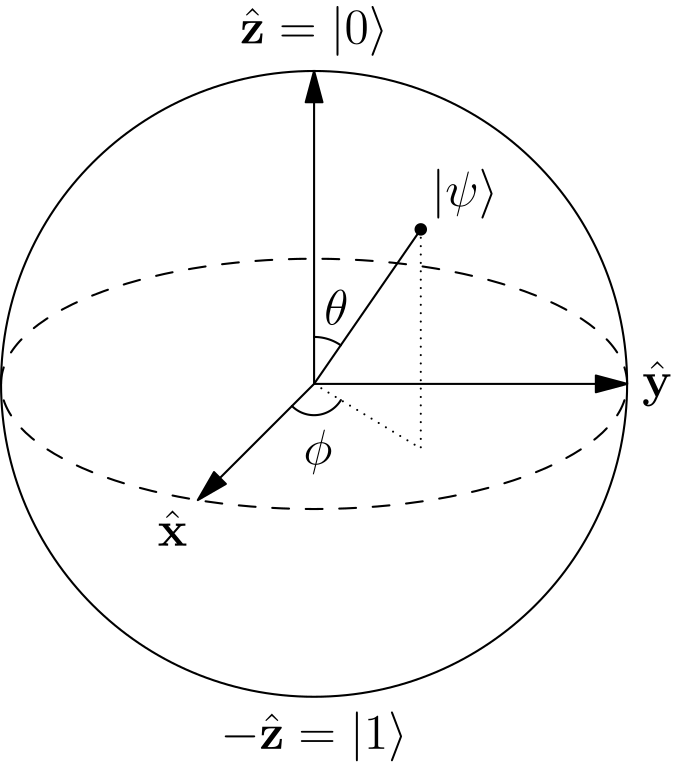
\includegraphics[width=0.4\linewidth]{Figures/677px-Bloch_Sphere.svg}
	\caption{Esfera de Bloch, on es representa un estat arbitrari $\ket{\psi}$ amb els vectors $\hat{\mathbf{x}}, \hat{\mathbf{y}}, \hat{\mathbf{z}}$ representat els eixos ortonormals de la esfera de radi $1$.}
	\label{fig:677px-blochsphere}
\end{figure}

%Glosser.ca, CC BY-SA 3.0 <https://creativecommons.org/licenses/by-sa/3.0>, via Wikimedia Commons
\subsection{Operacions per a només un qubit}
\label{only_one_qubit}
Una vegada la informació és representada amb els qubits, estaria bé poder operar amb aquesta informació. Operar amb la informació és justament el que fa que els ordinadors siguin ordinadors, poder operar amb la informació. En computació quàntica els qubits al poder ser representats amb vectors són operats per les anomenades portes lògiques quàntiques, que són matrius. Per exemple, si es vol passar de tindre un qubit en l'estat $\ket{0}$ a l'estat $\ket{1}$, s'utilitza la porta lògica $X$ representada a continuació:
$$
X = \begin{bmatrix}
	0 & 1\\
	1 & 0\\
\end{bmatrix}
$$ 
Podem veure com es fa aquesta l'acció al multiplicar la matriu pel vector:
$$
\begin{bmatrix} 0 & 1\\ 1 & 0\\ \end{bmatrix} \begin{bmatrix}1 \\ 0 \end{bmatrix} = \begin{bmatrix}0 \\ 1 \end{bmatrix}
$$
Que en notació de Dirac s'expressaria com: 
$$
X\ket{0} = \ket{1}
$$
D'una manera més general: 
$$
\begin{bmatrix} 0 & 1\\ 1 & 0\\ \end{bmatrix} 
\begin{bmatrix}\alpha \\ \beta \end{bmatrix} =
\begin{bmatrix} 0\times\alpha + 1\times\beta \\1\times\alpha + 0\times\beta \\
\end{bmatrix}
= \begin{bmatrix} \beta \\ \alpha \end{bmatrix}
$$
Es pot veure que aquesta matriu el que fa és donar la volta als coeficients d'un vector, per tant:
$$
X\ket{0} = \ket{1} \text{ i } X\ket{1} = \ket{0}
$$

Aquesta porta lògica forma part d'un grup de matrius molt important , les matrius de Pauli, compost  per 3 matrius: la X, la Y i la Z, usualment representades per $X$, $Y$, $Z$ o per $\sigma_x, \sigma_y, \sigma_z$. Aquestes matrius són les següents:
$$
	 X = \begin{bmatrix} 0 & 1\\ 1 & 0\\ \end{bmatrix} \; Y = \begin{bmatrix} 0 & i\\ -i & 0\\ \end{bmatrix} \; Z = \begin{bmatrix} 1 & 0\\ 0 & -1\\ \end{bmatrix} 
$$

Aquestes matrius són molt importants en la mecànica quàntica\footnote{Al ser Hermitianes són uns observables, concretament són els observables que corresponen al spin d'una partícula amb spin $\frac{1}{2}$ bàsicament estan relacionades amb els operadors del moment angular.} i són utilitzades àmpliament per descompondre portes lògiques quàntiques \cite{QCandQI:pauli}.

A partir d'elles podem elaborar matrius que facin una rotació d'un angle $\theta$ \cite{QCandQI:pauli} qualsevol en un dels eixos de la representació geomètrica d'un qubit \ref{fig:677px-blochsphere}:
\begin{align}
	& R_x(\theta) =  e^{-i\theta X/2} = \cos \frac{\theta}{2}I -i \sin \frac{\theta}{2}X = 
	\begin{bmatrix}
		\cos \frac{\theta}{2} & -i \sin \frac{\theta}{2} \\
		-i\sin \frac{\theta}{2} & \cos\frac{\theta}{2} \\
	\end{bmatrix} \label{eq:rx}\\
	& R_y(\theta) =  e^{-i\theta Y/2} = \cos \frac{\theta}{2}I -i \sin \frac{\theta}{2}Y = 
	\begin{bmatrix}
		\cos \frac{\theta}{2} & -\sin \frac{\theta}{2} \\
		\sin \frac{\theta}{2} & \cos\frac{\theta}{2} \\
	\end{bmatrix} \label{eq:ry}\\
	& R_z(\theta) =  e^{-i\theta Z/2} = \cos \frac{\theta}{2}I -i \sin \frac{\theta}{2}Z = 
	\begin{bmatrix}
		e^{-i\theta/2} & 0 \\
		0 & e^{i\theta/2} \\
	\end{bmatrix} \label{eq:rz}
\end{align}
Per exemple la matriu $R_y(\cdot)$ (Eq.\ref{eq:ry}) correspon a una rotació en l'eix $\hat{\mathbf{y}}$ de l'esfera de la figura \ref{fig:677px-blochsphere}.

Aquestes operacions poden resultar en superposicions si es fan rotacions amb certs angles. Però hi ha una porta lògica especial per poder fer una rotació que resulta en una superposició uniforme. És a dir una superposició que tingui les mateixes probabilitats de resultar en $\ket{0}$ o $\ket{1}$. Aquesta és la porta de Hadamard, denotada per $H$:
\begin{equation}
	H = \frac{1}{\sqrt{2}}\begin{bmatrix}
		1 & 1 \\ 1 & -1
	\end{bmatrix}
\end{equation}
Podem comprovar que és una superposició uniforme al aplicar-la a l'estat $\ket{0}$:
$$
H\ket{0} = \frac{1}{\sqrt{2}}\begin{bmatrix}1 & 1 \\ 1 & -1 \end{bmatrix}\begin{bmatrix}1 \\ 0\end{bmatrix} = \begin{bmatrix} \frac{1}{\sqrt{2}} \\ \frac{1}{\sqrt{2}} \end{bmatrix}
$$
L'estat resultant és un estat especial que s'escriu com $\ket{+}$\footnote{Un altre estat similar és $\frac{\ket{0} - \ket{1}}{\sqrt{2}}$, quan la matriu $H$ s'aplica a l'estat $\ket{1}$.}. La probabilitat que un estat col·lapsi en una determinada base és el coeficient de la seva base elevat al quadrat. Com que l'estat és:
$$
\ket{+} = \begin{bmatrix} \frac{1}{\sqrt{2}} \\ \frac{1}{\sqrt{2}} \end{bmatrix} = \frac{\ket{0} + \ket{1}}{\sqrt{2}} =  \frac{1}{\sqrt{2}}\ket{0} +  \frac{1}{\sqrt{2}}\ket{1}
$$
Al elevar al quadrat qualsevol dels coeficients es pot veure que dona $\frac{1}{2}$:
$$
\left(\frac{1}{\sqrt{2}}\right)^2 = \frac{1}{2}
$$
Llavors tenim que la probabilitat per obtenir els dos estats és la mateixa, és a dir que si mesurem l'estat $\ket{+}$ hi ha la mateixa probabilitat que surti $\ket{0}$ o $\ket{1}$. La porta lògica de Hadamard és molt important, ja que s'utilitza per crear distribucions uniformes, sigui en un qubit o en diversos\footnote{S'aplica aquesta operació a cada qubit del sistema.}.

Altres operacions importants de només un qubit són les portes $S$ i $T$:
$$
S=\begin{bmatrix} 1 & 0 \\ 0 & 1 \end{bmatrix} \; T=\begin{bmatrix} 1 & 0 \\ 0 & e^{i\pi/4} \end{bmatrix}
$$


\subsection{Circuit quàntics}
Aquestes operacions usualment es representen a través de circuits quàntics. Són representacions gràfiques que indiquen quines operacions s'apliquen a quins qubits i en quin ordre.

La forma de representar una porta $H$ aplicada a un qubit és amb el circuit quàntic:
\begin{center}
	\begin{quantikz}
		\lstick{$\ket{0}$} & \gate{H} & \qw
	\end{quantikz}
\end{center}

El qubit és representat per la línia que comença amb $\ket{0}$, amb $\ket{0}$ sent el seu estat inicial. Aquests diagrames es llegeixen d'esquerra a dreta, la mateixa forma en la qual s'apliquen les operacions.

Un qubit en el qual se li aplica una porta $H$ i després una porta $X$, és representat com:
\begin{center}
	\begin{quantikz}
		\lstick{$\ket{0}$} & \gate{H} & \gate{X} & \qw
	\end{quantikz}
\end{center}

Múltiples qubits són simplement més línies, aquí estan representant dos qubits amb portes $X$ aplicades a cada un:
\begin{center}
	\begin{quantikz}
		\lstick{$\ket{0}$} & \gate{X} & \qw \\
		\lstick{$\ket{0}$} & \gate{X} & \qw 
	\end{quantikz}
\end{center}

Amb els circuits quàntics també s'expressa l'ordre en el qual s'apliquen les portes, de esquerra a dreta. Un circuit de dos qubits, en el qual s'aplica una porta H en l'eix $x$ en el segon qubit, seria:
\begin{center}
	\begin{quantikz}
		\lstick{$\ket{0}$} & \gate{H} & \qw& \qw \\
		\lstick{$\ket{0}$} & \qw & \gate{R_x(\theta)} & \qw
	\end{quantikz}
\end{center}
Es pot veure que hi ha un ordre específic per aplicar aquestes portes, primer s'aplica la $H$ i després la rotació. 


\subsection{Operacions per a múltiples qubits}
El realment interessant és l'aplicació d'una porta a diversos qubits, perquè d'aquesta manera es pot arribar a tindre qubits entrellaçats. La porta més útil per entrellaçar qubits és la $\mathrm{CNOT}$ o \textit{Controlled NOT}:
\begin{equation}
	\mathrm{CNOT} = 
	\begin{bmatrix}
		1 & 0 & 0 & 0 \\
		0 & 1 & 0 & 0 \\
		0 & 0 & 0 & 1 \\
		0 & 0 & 1 & 0 \\
	\end{bmatrix}
\end{equation}

Aquesta porta s'aplica a dos qubits, que anomenaré $c$ i $t$. És bàsicament una porta $X$ que està controlada pel qubit $c$: si $c$ és $\ket{1}$, s'aplica la porta $X$ al qubit $t$. El cas contrari, amb el qubit $c$ sent l'estat $\ket{0}$, en el qubit $t$ no s'aplicaria cap porta.

Però si el qubit $c$ està en superposició, aquesta superposició passa també al qubit $t$, i al mesurar-lo, la probabilitat de què s'hagi aplicat la porta $X$ al qubit $t$ és la mateixa probabilitat de què $c$ estigui en l'estat $\ket{1}$. Els qubits d'alguna manera han passat a compartir la superposició. Es considera que aquests qubits estan entrellaçats, una mesura a un d'ells afecta a la mesura de l'altre. 

El qubit al qual se li aplica la porta $X$ es diu \textit{target} (que en l'explicació anterior seria el qubit $t$) i el qubit sobre el qual depèn el \textit{target} és el \textit{control} (que seria el qubit $c$).

Aquesta porta representada en un circuit s'escriu com\footnote{A vegades escriuré els circuits quàntics sense especificar l'estat inicial, ja que no és necessari.}:
\begin{center}
	\begin{quantikz}
		& \ctrl{1} & \qw \\
		& \targ{} & \qw
	\end{quantikz}
\end{center}
On el qubit \textit{control} és el primer i el segon és el \textit{target}, el qubit que té el símbol $\oplus$.


\subsubsection{Entrellaçament quàntic}
L'exemple més senzill d'un entrellaçament quàntic en la computació quàntica són els parells de Bell. Es creen al aplicar a dos qubits una porta $H$ al primer i després una porta $\mathrm{CNOT}$ als dos creant l'estat \cite{QCandQI:entangle}:
$$
\frac{\ket{00}+\ket{11}}{\sqrt{2}} = \frac{1}{\sqrt{2}}\ket{00} + \frac{1}{\sqrt{2}}\ket{11}
$$
Es pot veure que només hi ha dos estats possibles $\ket{00}$ i $\ket{11}$ que tenen la mateixa probabilitat associada\footnote{Això es pot veure a l'elevar al quadrat els coeficients del dos, que donen $\frac{1}{2}$.}. S'afecten l'un a l'altre en el sentit que quan es mesura només un dels qubits i dona per exemple $\ket{1}$, al mesurar l'altre també donaria $\ket{1}$. D'aquesta manera acabant amb l'estat $\ket{11}$. En altres paraules, la mesura d'una part del sistema determina el resultat d'una mesura en una altra part del sistema.

Matemàticament, un sistema quàntic, i.e. un conjunt de qubits, està entrellaçant quan aquest sistema no es pot descriure amb un producte tensorial de les parts. Per exemple estat $\ket{00}$ es pot escriure com $\ket{0}\otimes\ket{0}$, mentre que l'estat $\frac{\ket{00} + \ket{11}}{\sqrt{2}}$, no. Per tant, el primer no és sistema amb qubits entrellaçats i el segon sí ho és.

A partir de l'entrellaçament i la superposició és com els ordinadors quàntics arriben a tenir avantatges en complexitat sobre els ordinadors clàssics, per a més informació sobre els avantatges que presenten els algoritmes quàntics en certes tasques i el concepte de complexitat algorítmica veure l'annex \ref{complexity}.

\subsubsection{Operacions controlades}
A part de la porta $\mathrm{CNOT}$ existeixen diverses portes quàntiques controlades. Realment es pot controlar qualsevol porta, en altres paraules, si l'estat del qubit \textit{control} és $\ket{0}$, s'aplica qualsevol porta al qubit \textit{target}. Fins i tot poden haver-hi diversos qubits \textit{control} i \textit{target} \cite{QCandQI:controlled}.

Per exemple existeix la porta Toffoli:
\begin{center}
	\begin{quantikz}
		& \ctrl{1} & \qw \\
		& \ctrl{1} & \qw \\
		& \targ{} & \qw
	\end{quantikz}
\end{center}
La seva forma matricial és:
$$
\begin{bmatrix}
	1 & 0 & 0 & 0 & 0 & 0 & 0 & 0 \\
	0 & 1 & 0 & 0 & 0 & 0 & 0 & 0 \\
	0 & 0 & 1 & 0 & 0 & 0 & 0 & 0 \\
	0 & 0 & 0 & 1 & 0 & 0 & 0 & 0 \\
	0 & 0 & 0 & 0 & 1 & 0 & 0 & 0 \\
	0 & 0 & 0 & 0 & 0 & 1 & 0 & 0 \\
	0 & 0 & 0 & 0 & 0 & 0 & 0 & 1 \\
	0 & 0 & 0 & 0 & 0 & 0 & 1 & 0 \\
\end{bmatrix}
$$
Aquesta porta aplica una porta $X$ a l'últim qubit en cas que els dos primers siguin $\ket{0}$.

Tornant a dos qubits, al veure la matriu per la porta $\mathrm{CNOT}$, es pot apreciar que està composta per una matriu identitat i una porta $X$\footnote{La matriu identitat es troba a la cantonada superior esquerra, mentre que la porta $X$ es troba a l'altre extrem.}:
$$
\begin{bmatrix}
	1 & 0 & 0 & 0 \\
	0 & 1 & 0 & 0 \\
	0 & 0 & 0 & 1 \\
	0 & 0 & 1 & 0 \\
\end{bmatrix}
$$
També al veure la porta $Z$ controlada ($\mathrm{CZ}$), es pot apreciar el mateix patró:
$$
\begin{bmatrix}
	1 & 0 & 0 & 0 \\
	0 & 1 & 0 & 0 \\
	0 & 0 & 1 & 0 \\
	0 & 0 & 0 & -1 \\
\end{bmatrix}
$$
Amb la matriu de la porta $Z$ a la cantonada inferior dreta. Aquesta porta en un circuit quàntic es representa de la següent manera:
\begin{center}
	\begin{quantikz}
		& \ctrl{1} & \qw \\
		& \control{} & \qw
	\end{quantikz}
\end{center}

Una operació controlada de qualsevol matriu unitària $U$ es pot formar a través del següent circuit \cite{QCandQI:controlled}:
\begin{center}
	\begin{quantikz}
		& \ctrl{1} & \qw \\
		& \gate{U} & \qw
	\end{quantikz}
	=
	\begin{quantikz}[align equals at=1.5, column sep=0.3cm]
		& \qw & \ctrl{1} & \qw & \ctrl{1} & \gate{\begin{bmatrix}
				1 & 0 \\
				0 & e^{i\alpha}
		\end{bmatrix}}\\
		& \gate{C} & \targ{} & \gate{B} & \targ{} & \gate{A}
	\end{quantikz}
\end{center}

On $U, \alpha, A, B$ i $C$ son tals que $U = e^{i\alpha}AXBXC$ i  $ABC = I$.

\section{Mesurament quàntic}
Com ja s'ha esmentat a la secció \ref{only_one_qubit} a l'elevar al quadrat el coeficient d'un estat base que forma part d'un estat, s'obté la probabilitat d'obtenir aquest estat base quan es mesura. 

Aquesta és la forma més simple de poder predir el mesurament d'un estat quàntic. Però hi ha altres mètodes que a vegades resulten més útils.

Els mesuraments quàntics també es ponen pensar com un conjunt d'operadors de mesura ${M_m}$, on la probabilitat d'obtenir l'estat $m$ associat a un operador $M_m$ al mesurar un $\ket{\psi}$ és \cite{QCandQI:measure}:
\begin{equation}
	\label{eq:Mm}
	\mathrm{prob}(m)=\bra{\psi}M_{m}^\dagger M_{m}\ket{\psi}
\end{equation}

On l'estat després de la mesura és:
$$
\frac{M_{m}\ket{\psi}}{\sqrt{\bra{\psi}M_{m}^\dagger M_{m} \ket{\psi}}}
$$
Els operadors ${M_m}$ han de complir que las suma de les seves probabilitats sigui $1$:
$$
1 = \sum_m \mathrm{prob}(m) = \sum_m \bra{\psi}M_{m}^\dagger M_{m}\ket{\psi}
$$

La diferència entre aquesta manera de fer les mesures i elevar els coeficients al quadrat, és que l'equació \ref{eq:Mm} és una forma més general, on en comptes de mesurar en la base computacional, es pot mesurar en qualsevol base. 

Per mesurar en la base computacional d'un \textit{statevector} s'utilitzen operadors de mesura derivats de la base computacional fets a partir de productes exteriors. Per crear l'operador de mesura ${M_i}$ associat a la base computacional $\ket{i}$ s'agafa el producte exterior de la base:
$$
M_i = \ket{i}\bra{i}
$$
Per tant la probabilitat que la mesura de l'estat $\ket{\psi}$ resulti en $\ket{0}$, és:
\begin{align*}
	\mathrm{prob}(\ket{0}) &= \bra{\psi}M_{\ket{0}}^{\dagger}M_{\ket{0}} \ket{\psi}\\
	&= \bra{\psi}(\ket{0}\bra{0})^\dagger \ket{0}\bra{0}\ket{\psi} 
\end{align*}


Per $\ket{\psi} = \ket{0}$ tenim que\footnote{Cal notar que ($\ket{0}\bra{0})^\dagger = \ket{0}\bra{0}$ i que $\ket{0}$ és un vector unitari.}:
\begin{align*}
	\mathrm{prob}(\ket{0}) &= \bra{0}\ket{0}\bra{0}^\dagger \ket{0}\bra{0}\ket{0} \\
	&= \bra{0}\ket{0}\bra{0} \ket{0}\bra{0}\ket{0} \\
	&= \bra{0}\ket{0}\bra{0}\ket{0} \\
	&= 1
\end{align*}
El resultat té sentit, ja que si mesurem $\ket{0}$ en la base $\ket{0}$, la probabilitat de trobar l'estat hauria de ser $1$.

\section{Matriu de densitat}
Una sèrie de qubits es pot representar tant per un vector com per una matriu, anomenats vector d'estat i matriu de densitat, respectivament \cite{QCandQI}.
En aquesta secció explicaré ràpidament sobre el concepte de matriu de densitat i com les operacions que s'apliquen a un vector d'estat poden ser aplicades a aquesta matriu. Després parlaré dels mesuraments parcials d'un sistema, un concepte que és important per la part experimental del treball.

Una matriu de densitat és la representació matemàtica d'un estat quàntic a partir d'una matriu. Aquest concepte en anglès s'anomena \textit{density operator/matrix}. Aquesta representació serveix per descriure sistemes quàntics que no són completament coneguts. Concretament, aquestes matrius són conjunts d'estats quàntics: Per un sistema que es descriu com un conjunt d'estats $\{\ket{\psi_i}\}$ amb cada element del conjunt té una probabilitat associada de $p_i$. La matriu densitat $\rho$ del d'aquest sistema és \cite{QCandQI:density_matrix}:
$$
\rho = \sum_i p_i\ket{\psi_i}\bra{\psi_i}
$$
Aquesta matriu pot ser simplement $\ket{\psi}\bra{\psi}$ per un estat qualsevol $\ket{\psi}$, per exemple la matriu que representa $\ket{0}$ és:
$$
\rho = \ket{0}\bra{0} = \begin{bmatrix}
	1 & 0 \\
	0 & 0 
\end{bmatrix}
$$

L'evolució d'un operador de densitat que descriu un sistema quàntic, igual que amb els vectors, s'efectua a partir de matrius unitàries. Un estat $\rho$ evoluciona partir d'una matriu unitària $U$ de la següent manera:
$$
\sum_i p_i U \ket{\psi_i}\bra{\psi_i} U^\dagger = U\rho U^\dagger 
$$

Igual que es fan mesures en els \textit{statevectors}, les podem fer en els operadors de densitat. Per un operador de mesura $M_m$, tenim que la probabilitat de tindre l'estat $m$ al mesurar un vector $\ket{\psi}$ o una matriu de densitat $\rho$, és:
\begin{align*}
	\mathrm{prob}(m) &= \bra{\psi}M_m^\dagger M_m\ket{\psi} = \Tr(M_m^\dagger M_m \ket{\psi}\bra{\psi})\\ &= \Tr(M_m^\dagger M_m \rho)
\end{align*}
També tenim que l'estat $\ket{\psi}$ després de la mesura $m$ és \cite{QCandQI:density_matrix}:
\begin{equation}
	\ket{\psi_{m}} = \frac{M_m\ket{\psi}}{\sqrt{\bra{\psi}M_m^\dagger M_m \ket{\psi}}} = \frac{M_m\ket{\psi}}{\sqrt{\Tr(M_m^\dagger M_m \rho)}}
	\label{eq:post_state_rho}
\end{equation}

L'equació \ref{eq:post_state_rho} es pot reescriure en termes d'una matriu de densitat després d'una mesura $m$:
\begin{align*}
	\rho_m &= \sum_i p_i \frac{M_m\ket{\psi}\bra{\psi}M_m^\dagger}{\Tr(M_m^\dagger M_m \rho)} \\
	&= \frac{M_m\rho M_m^\dagger }{\Tr(M_m^\dagger M_m\rho)}
\end{align*}
Perquè això sigui cert els operadors de mesura $M_m$, han de satisfer:
$$
\sum_m M_m^\dagger M_m = I
$$
Per a tots els estats possibles $m$.

Per últim s'ha de recordar que les matrius densitat igual que els vectors d'estat han de tenir certes característiques:
\begin{enumerate}
	\item La traça de $\rho$ ha d'equivaldre a $1$.
	\item $\rho$ ha de ser un operador positiu\footnote{Un operador positiu $A$ es aquell que $\bra{\psi}A\ket{\psi}\geq0, \forall \ket{\psi}$.}.
\end{enumerate}
\subsection{Matriu de densitat reduïda}
Una aplicació important dels operadors de densitat és la descripció d'estats parcials amb l'operador de densitat reduït, i per tant, la descripció dels mesuraments parcials.

Per un sistema físic compost per dos sistemes $A$ i $B$ que es descriu per una matriu de densitat $\rho^{AB}$, la matriu de densitat reduïda del sistema $A$ és:
\begin{equation}
\rho^A = \Tr_B(\rho^{AB})
	\label{eq:partial_trace}
\end{equation}
On $\Tr_B$ és la traça parcial sobre el sistema $B$, que es defineix per l'equació següent \cite{QCandQI:partial_trace}: 
\begin{equation*}
	\Tr_B(\ket{a_1}\bra{a_2}\otimes\ket{b_1}\bra{b_2}) = \ket{a_1}\bra{a_2}\Tr(\ket{b_1}\bra{b_2})
\end{equation*}
Amb $\ket{a_1}$ i $\bra{a_2}$ sent estats vàlids pel sistema $A$, i $\ket{b_1}$ i $\bra{b_2}$ sent-ho per $B$. El terme $\Tr(\ket{b_1}\bra{b_2})$ s'omet quan els vectors del producte exterior són iguals i formen un operador de densitat vàlid, el qual té una traça de $1$.

No obstant aquesta definició no es pot utilitzar quan no saps com representar la matriu de densitat $\rho$ com a un producte tensorial, en el qual un dels termes és l'estat que es traça a fora. En altres paraules, en l'equació \ref{eq:partial_trace} si no es coneix $\rho^A$ i $\rho^B$ per $\rho^{AB} = \rho^A\otimes\rho^B$, aquesta equació no serveix de res.

A causa d'això en el llibre de text \textit{Quantum Computing: A Gentle Introduction} \cite{QC_intro} els autors defineixen la traça parcial d'una altra manera més general, on només s'ha de saber les bases dels sistemes $A$ i $B$ i un operador vàlid pel sistema $AB$. Per una matriu de densitat $\rho^{AB}$ que representa un estat del sistema $A\otimes B$, la traça parcial de $\rho^{AB}$ sobre $B$ és:
$$
\Tr_B \rho^{AB} = \sum_i \bra{\beta_i}\rho^{AB}\ket{\beta_i}
$$
On el conjunt $\{ \ket{\beta_i} \}$ són les bases del sistema $B$. Les entrades de la matriu $\Tr_B \rho^{AB}$ representades en termes de les bases ${\ket{\alpha_i}}$ i ${\ket{\beta_j}}$ dels sistemes $A$ i $B$ respectivament, són:
$$
(\Tr\rho^{AB})_{ij} = \sum_{k=0}^{M-1} \bra{a_i}\bra{\beta_k}\rho^{AB}\ket{\alpha_j}\ket{\beta_k}
$$
Amb la matriu sent:
$$
\Tr\rho^{AB} = 
\sum_{i,j=0}^{N-1}\left(\sum_{k=0}^{M-1} \bra{a_i}\bra{\beta_k}\rho^{AB}\ket{\alpha_j}\ket{\beta_k}\right) \ket{\alpha_i}\bra{\alpha_j}
$$
On $N$ és la dimensió del sistema $A$ i $M$ és la dimensió del sistema $B$. 

Es pot comprovar que aquestes definicions són correctes ja que en els dos llibres utilitzen les seves definicions per tractar el mateix cas i obtenen el mateix resultat \cite{QCandQI:example_partial, QC_intro:example_partial}.

\subsubsection{Mesurament parcial}
\label{par_measurament}
Es pot arribar a treure una mesura parcial\footnote{És a dir, una mesura a només una part dels qubits que conformen un sistema.} sobre un sistema de qubits amb la traça parcial i operadors de mesura. En el paper fet per Huang et.al. \cite{QGAN_exp} es descriu un estat $\rho$ després d'un mesurament parcial $\Pi_A$ sobre un sistema $A$ que pertany a l'estat $\ket{\psi}$ com:
$$
\rho = \frac{\Tr_A(\Pi_A \ket{\psi}\bra{\psi})}{\Tr(\Pi_A\otimes I_{2^N-2^{N_A}}\ket{\psi}\bra{\psi})}
$$
Essent $\Pi_{A}$ un mesurament parcial definit com\footnote{No estic completament segur d'això ja que els autors no defineixen aquest operador per aquesta equació en concret, però en un altre equació si que ho fan.} a $\Pi_{A}=(\ket{0}\bra{0})^{\otimes N_{A}}$, on $N_{A}$ és el nombre de qubits sobre els quals es treu el mesurament parcial.

El sistema $A$ al estar composts $N_A$ qubits, per tant, la resta de l'estat $\ket{\psi}$ té $N-N_A$, on $N$ és el nombre total de qubits del estat $\ket{\psi}$. D'aquesta manera $\Pi_A\otimes I_{2^N-2^{N_A}}$ té $2^N\times 2^N$ dimensions i pot ser multiplicat per la matriu $\ket{\psi}\bra{\psi}$ que té les mateixes dimensions. No obstant això, sorgeix un problema amb el numerador de l'equació perquè $\Pi_A$ no té les mateixes dimensions\footnote{En aquesta afirmació no tinc cap dubte, ja que no és necessita la definició de $\Pi_{A}$ per poder afirmar-ho.} que $\ket{\psi}\bra{\psi}$, encara no he pogut utilitzar aquesta equació adequadament. No sé com computar-la. Aquest problema l'adreçaré en la part experimental del treball.

En el mateix article es planteja una altra equació, per l'estat post-mesura expressat en forma de vector d'estat, molt semblant a l'equació \ref{eq:post_state_rho}. L'única diferencia és que en l'equació de l'article no s'expressa l'operador de mesura en la forma $M_m^\dagger M_m$, en canvi, els autors ho expressen tan sols com $I_{2^N-2^{N_A}}\otimes \Pi_A$. Potser la forma plantejada pels autors té en compte el conjugat hermitià, però no estic segur.
L'equació esmentada en l'article és la següent:
$$
\ket{\psi_m} = \frac{I_{2^N-2^{N_A}}\otimes\Pi_A\ket{\psi}}{\sqrt{\Tr(I_{2^N-2^{N_A}}\otimes\Pi_A\ket{\psi}\bra{\psi})}}
$$
Al igual que amb l'altra equació, no sé com computar-la\footnote{Un cop entregat el treball me pogut veure que si que la puc computar, no obstant això, no és pertinent fer canvis en la part experimental o les conclusions del treball amb aquesta nova informació. }.

\section{Ordinadors quàntics}
Tota aquesta teoria es veu plasmada a la realitat als qubits físics dels ordinadors quàntics. Hi ha diversos tipus d'ordinadors quàntics, a causa del fet que els qubits poden ser diversos sistemes. Poden ser fotons, xips de silici superconductors o ions atrapats per imants. No elaboraré més sobre aquest tema, ja que no és el tema central d'aquest treball, m'he centrat molt més en la teoria.

Però si vull generar imatges amb un ordinador quàntic, no en necessito un? No necessàriament, perquè puc simular l'evolució dels estats quàntics amb un ordinador, al cap i a la fi, és només àlgebra lineal, són operacions que es poden fer perfectament en un ordinador. No obstant això, quan s'intenta simular un sistema quàntic de molt qubits,\footnote{Més de 50 per exemple.} un ordinador de sobretaula tardaria molt de temps i realment no és viable fer-ho.


\chapter{Intel·ligència artificial}
\label{ML}
Segurament has sentit parlar de les intel·ligències artificials o de les xarxes neuronals, són conceptes que semblen abstractes, però jo penso que són bastant intuïtius i en aquest capítol els intentaré explicar de la millor manera possible.

Intel·ligència artificial és un mot una mica ambigu, que es refereix a qualsevol algoritme que entra dintre del camp del \textit{machine learning} o aprenentatge automàtic\footnote{Tanmateix, col·loquialment s'utilitza per denominar a qualsevol algoritme o robot que és intel·ligent o sembla que és intel·ligent. }. Aquests algoritmes simplement s'alteren a ells mateixos per fer millor la tasca que s'els ha designat. No importa quin és l'objectiu o com s'ha aconsegueix, el que importa és si aprèn automàticament. Cal notar que els canvis que s'efectuen els algoritmes sobre si mateixos no han de ser predeterminats, si l'algoritme té una llista de les instruccions que va executant segon la situació no seria una intel·ligència artificial o un algoritme d'aprenentatge automàtic.  \cite{deeplearning}.

La manera que tenen aquests algoritmes d'alterar-se a si mateixos és canviant els paràmetres de les operacions dels quals estan compostos. Això ho fan a partir de veure patrons en un conjunt de dades. Per exemple, en una regressió lineal, s'actualitzen els paràmetres de la recta que representa la tendència de les dades, com es pot veure a la figura \ref{fig:leastsquares}.

\begin{figure}
	\centering
	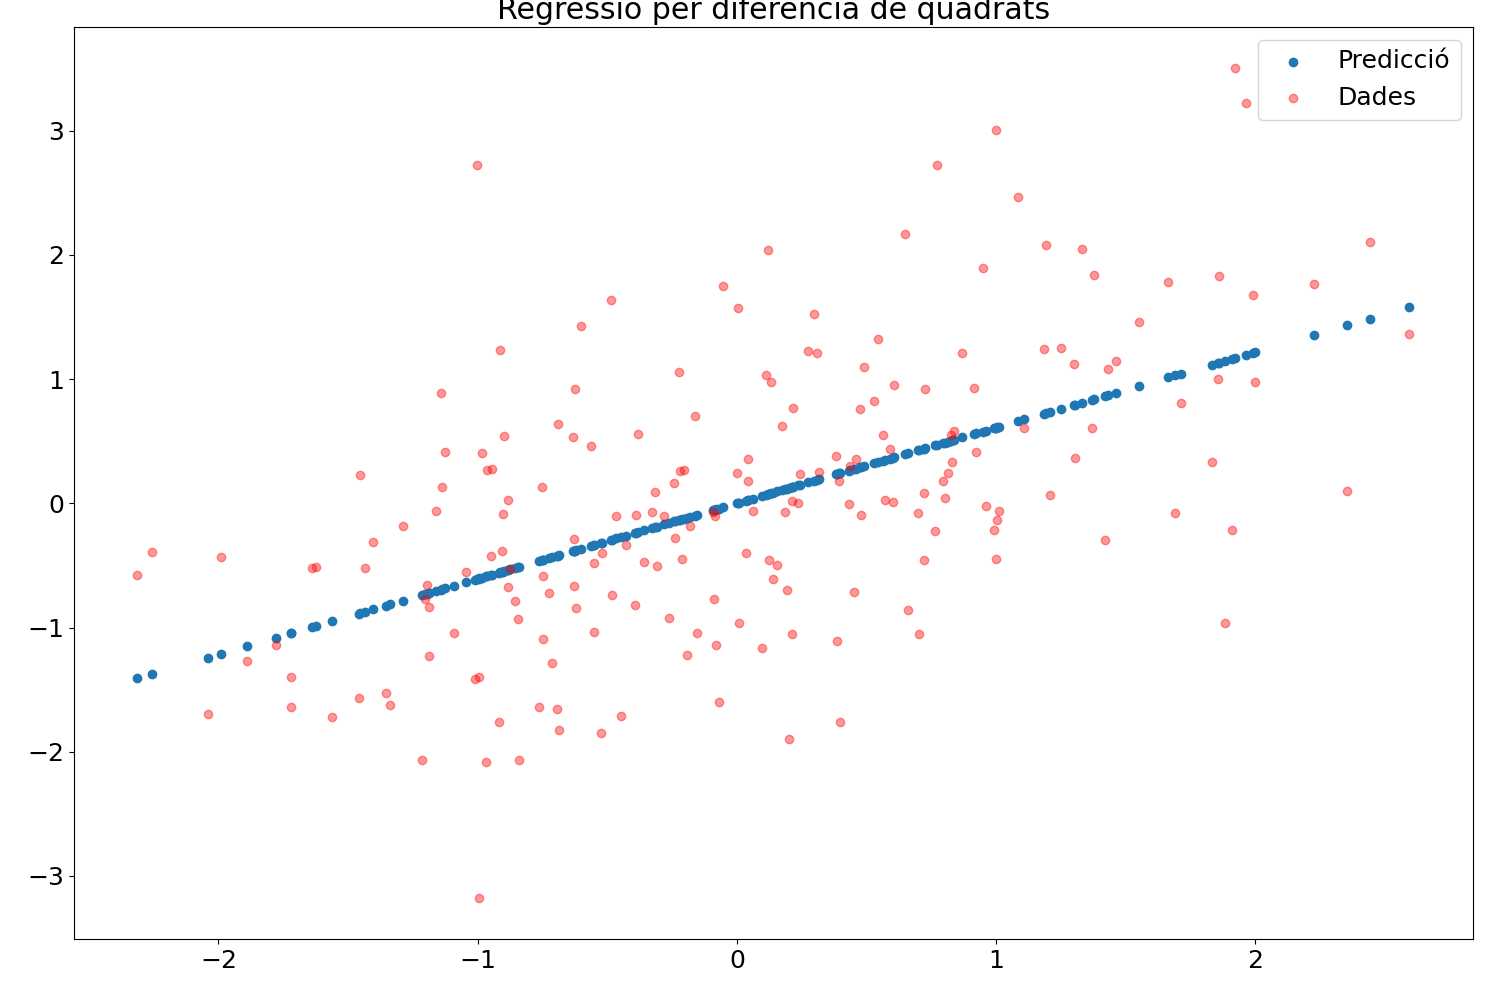
\includegraphics[width=0.7\linewidth]{Figures/least_squares}
	\caption{Exemple d'una regressió lineal de dades generades a l'atzar. Veure el codi a \ref{lst:linear_regression}.}
	\label{fig:leastsquares}
\end{figure}

Per ajustar els paràmetres, el més comú és ajustar-los segons la derivada d'una funció anomenada funció de pèrdua o \textit{loss function}, usualment representada per la lletra $\mathcal{L}$. Aquesta funció representa els objectius del programa i pot ser minimitzada o maximitzada. Per exemple, en una regressió lineal es vol reduir la distància entre els punts de dades i la línia que prediu la tendència.

A causa de que de la gran varietat de funcions de pèrdua que existeixen, els programes de \textit{machine learning} són extremadament versàtils. La màxima expressió d'això es pot veure en les xarxes neuronals o \textit{neural networks}, on les diverses arquitectures de xarxes neuronals que existeixen també contribueixen a la seva versatilitat \cite{deeplearning}. 

Aquests algoritmes són els més potents, complexos i polivalents, dintre de l'aprenentatge automàtic. Precisament utilitzo un d'aquests algoritmes d'aquests per generar les imatges. Es fan servir, entre altres coses, pel reconeixement d'imatges, la traducció i sintetització de textos, la conducció automàtica, els algoritmes de recomanació, i és clar, la generació d'imatges.

\section{Xarxes neuronals}
Aquests tipus d'algoritmes tenen un nom que fa recordar a les xarxes de neurones dels nostres cervells; no és casualitat, ja que estan directament inspirades en els nostres cervells. Són uns programes que consisteixen en la connexió de diverses operacions anomenades neurones, que conjuntament formen una xarxa, la qual s'organitza a partir de capes. Segons la variació del tipus de neurona i l'estructura que aquestes formen, podem tindre algoritmes destinats a fer diferents tasques. Això juntament amb els diversos tipus de funció de pèrdua contribueix a la versatilitat de les xarxes neuronals. Aquests models d'intel·ligència artificial constitueixen el camp del \textit{deep learning} o aprenentatge profund. S'anomenen d'aquesta forma per referenciar la gran profunditat d'aquests algoritmes, és a dir el gran nombre de capes que tenen \cite{DL:feedforward}.

Una neurona consisteix simplement en una suma ponderada, a la qual se li suma un altre número, i finalment una funció no lineal que s'aplica al resultat. Les neurones tenen vectors com input i output. Per tant, una neurona es pot definir com:
$$
\sigma \left(\sum_{i=1}^n w_i x_i + b\right) = \sigma \left( w_1x_1 + w_2x_2 + \cdots + w_nx_n + b 
\right) 
$$
Essent $\sigma$ sent una funció no lineal i $n$ la mida del vector. Després estan els paràmetres, $w_i$ i $b$, anomenats \textit{weights} i \textit{bias}.

Una neurona pot tindre diversos inputs que venen de diverses neurones; el mateix passa amb els outputs. Depenent de com es connectin entre si les neurones, aquestes passen a formar diversos tipus de capes. A partir dels tipus de capes i el nombre d'aquestes és com s'especifica l'arquitectura d'una xarxa neuronal.

Una vegada especificada la interconnectivitat de les neurones puc parlar de la intuïció darrere dels paràmetres. Un \textit{weight} especifica com és de forta la relació entre una neurona en una capa i una altra neurona en una capa veïna. I un \textit{bias} especifica com és d'important una neurona, ja que aquest número afecta el resultat a la suma, fent que l'activació de la neurona\footnote{Així és com s'anomena el seu resultat.} sigui més alta.

Tornant a l'arquitectura, usualment aquesta es divideix en tres parts la capa d'input, les capes ocultes i la capa d'output. La quantitat de neurones que hi ha a la capa d'inputs és la que defineix la mida del vector que es dona com input a la xarxa, ja que cada element del vector es dona a cada neurona amb la capa. El mateix passa amb la capa d'outputs, cada output de cada neurona de la capa acaba sent un element en el vector que surt de la xarxa. Per tant, el nombre de neurones que té cadascuna d'aquestes dues capes, especifica la mida dels vectors d'input i d'output de la xarxa respectivament. Per exemple, si es vol donar com input a una xarxa una imatge de 16 per 16 píxels en blanc i negre calen 256 neurones en la capa d'inputs, una per cada píxel.

En canvi, les \textit{hidden layers}, és a dir les capes ocultes, no tenen una mida determinada, el mateix passa amb el nombre d'aquestes que té la xarxa. Depenen de cada cas la quantitat de neurones que tenen aquestes capes i també el nombre d'aquestes, varia. Això, juntament amb els diversos tipus de capes és el que dona la versatilitat d'aquests algoritmes \cite{DL:feedforward}.

Entre els diferents tipus de capes que ponen tindre les xarxes neuronals, la més comuna i simple d'aquestes és la \textit{fully connected layer}, o una capa completament connectada, com les que es poden veure en la figura \ref{fig:560px-artificialneuralnetwork}. Les neurones que formen aquesta capa estan connectades a totes les neurones de la capa anterior i així mateix, a totes les neurones de la capa següent. L'única forma que aquestes capes tenen de variar és a partir de canviar el nombre de neurones, ja que no es pot alterar el funcionament de les neurones.
\begin{figure}[H]
	\centering
	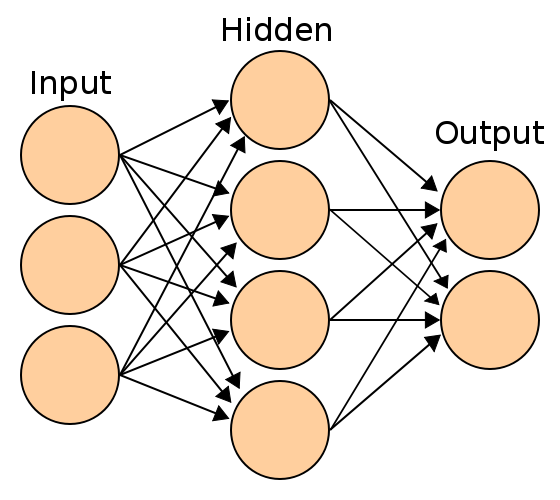
\includegraphics[width=0.7\linewidth]{Figures/560px-Artificial_neural_network.svg}
	\caption{Usualment, les xarxes neuronals es representen d'aquesta forma, amb fletxes i boles. Les boles representarien cada neurona i les fletxes mostren com estan connectades. La \textit{hidden layer} d'aquesta representació es pot veure que és una \textit{fully connected layer} a causa de com està connectada a les altres capes, rebent cada neurona l'output de cada neurona anterior.}
	\label{fig:560px-artificialneuralnetwork}
	% en:User:Cburnett, CC BY-SA 3.0 \href{http://creativecommons.org/licenses/by-sa/3.0/}, via Wikimedia Commons
\end{figure}
No obstant això, es pot variar la funció d'activació que tenen, que ha de ser una funció no lineal. La més utilitzada és la sigmoide:
$$
f(x) = \frac{1}{1+e^{-x}}
$$

\section{Descens del gradient}
\label{gradient_descent}
Una vegada he parlat de les xarxes neuronals, he de comentar com aquestes evolucionen al llarg del temps, és a dir com se'n van actualitzen a si mateixes per complir el seu objectiu. Ja he comentat que existeix una funció anomenada \textit{loss function}, la qual es deriva per actualitzar els paràmetres de la xarxa. El mecanisme pel qual s'actualitzen els paràmetres s'anomena el descens del gradient.

Aquest procés comença amb la funció de pèrdua, que esmenta els objectius de la xarxa. Els punts mínims d'aquesta funció representen els punts òptims de la xarxa, als quals es vol arribar. 

 Per explicar-lo utilitzaré un exemple pràctic, primer de tot parlaré sobre la funció de pèrdua que s'utilitza i a continuació de l'actualització dels paràmetres. 
 
Parlaré de la classificació d'imatges, si es volen classificar imatges de gats i gossos, s'assignen dues etiquetes a aquestes, per exemple, $1$ als gats i $0$ als gossos. A continuació s'escull una funció de pèrdua\footnote{Una que funcioni per la classificació d'imatges, és clar.} com \textit{binary cross entropy} o \textit{log loss}. La funció \textit{binary cross entropy} és la següent \cite{crossentropy}:
\begin{equation}
	\mathcal{L} = - t\log(y) - (1 - t)\log(1 - y) 
	\label{eq:BCE}
\end{equation}
Amb $t$ sent l'etiqueta que ha de tenir la imatge, anomenada etiqueta real, i $y$ sent l'etiqueta que el model assigna a la imatge. Per tant, si l'etiqueta real és $1$, l'equació acaba sent \cite{crossentropy}:
$$
\mathcal{L}_1 = - \log(y)
$$
I el cas contrari per $t = 0$ seria:
$$
\mathcal{L}_0 = - \log(1 - y)
$$

Si donen com input la imatge d'un gat i el programa es dona com output $0.92$ tenim que la pèrdua és de:
\begin{align*}
	\mathcal{L} &= - t\log(y) - (1 - t)\log(1 - y) = - \log(0.92) \simeq 0.0834
\end{align*}
En canvi, si el programa es dona un output de $0.15$ la pèrdua, seria:
\begin{align*}
	\mathcal{L} &= - t\log(y) - (1 - t)\log(1 - y) = - \log(0.15) \simeq 1.897
\end{align*}
Es pot veure que si l'etiqueta que posa el model s'allunya més de l'etiqueta real la pèrdua acaba sent més gran. El mateix es pot veure per les imatges dels gossos, és a dir, les imatges que haurien de tenir etiqueta zero:
\begin{align*}
	\mathcal{L} &= - 0\cdot\log(0.89) - (1 - 0)\cdot\log(1 - 0.89) = - \log(1- 0.89) \simeq 2.207 \\
	\mathcal{L} &= - 0\cdot\log(0.08) - (1 - 0)\cdot\log(1 - 0.08) = - \log(1- 0.08)\simeq 0.0834
\end{align*}
Per tant, com més pròximes estiguin les prediccions (els outputs del model) a les etiquetes ideals, menor serà la pèrdua. Llavors al minimitzar la funció es trobarà el punt òptim on totes les prediccions seran iguals a les etiquetes \cite{DL:minmax}.

A aquests punts òptims s'arriben actualitzant els paràmetres a partir de la derivada de la funció, concretament a través del seu gradient. El gradient d'una funció és un vector on els seus elements són la derivada parcial respecte a cada paràmetre (per aclarir, una entrada per paràmetre). El gradient d'una funció $f(\theta)$ es representa com $\nabla f(\theta)$, i es pot escriure en forma de vector com:
$$
\nabla f(\theta) = \begin{bmatrix}
	\pdv{f}{\theta_1} \\
	\pdv{f}{\theta_2} \\
	\vdots \\
	\pdv{f}{\theta_{n-1}} \\
	\pdv{f}{\theta_{n}}
\end{bmatrix}
$$
No fa falta fixar-se en el que és exactament un gradient, només s'ha de saber que cada paràmetre de la xarxa neuronal\footnote{Cada \textit{weight} i cada \textit{bias}.} s'ha d'actualitzar d'acord amb la derivada respecte al paràmetre. Això es pot entendre com canviar lleugerament un paràmetre d'acord amb la direcció de la derivada respecte a ell. L'objecte que s'encarrega d'actualitzar-los s'anomena optimitzador. L'optimitzador més senzill que hi ha és el següent \cite{3b1b}:
\begin{equation}
	\theta_{i}^t = \theta_{i}^{t-1} \pm \eta\pdv{\mathcal{L}(\theta)}{\theta_{i}^{t-1}}
	\label{eq:optimizator}
\end{equation}
Es pot veure com s'actualitza el paràmetre $\theta_i$. En l'equació he posat el superíndex $t$ per expressar aquesta actualització, passant d'un temps $t-1$ a $t$. També, utilitzo el símbol $\theta$ per expressar tots els paràmetres del model, que es troben en la forma d'un vector. En els optimitzadors s'afegeix un nombre $\eta$ anomenat \textit{learning rate}. Usualment, és un nombre petit\footnote{Entre $0.1$ i $0.001$ per exemple.}, aquest nombre especifica com de ràpid canvien els paràmetres. El \textit{learning rate} es pot anar ajustant depenen de la situació o del model en el qual s'implementi. Alteracions en aquest poden causar diversos fenòmens tant negatius com positius, i aquesta és la principal tasca que tenen els optimitzadors, alterar el \textit{learning rate}. Existeixen molts optimitzadors que donen a terme aquesta tasca de diverses maneres, un dels més rellevants és ADAM \cite{adam}. 

Cal notar que en l'optimitzador he utilitzat el signe $\pm$ perquè si és positiu significa que s'està ascendint pel gradient, i si és negatiu s'està descendint. No obstant això, usualment es fa servir el signe negatiu per convenció, ja que la majoria de funcions de pèrdua estan dissenyades per ser minimitzades. 

Al fer la derivada de la funció de pèrdua es pot veure immediatament que s'ha d'aplicar la regla de la cadena, ja que l'estructura de la xarxa neuronal està composta per una sèrie de funcions compostes entre si. En la secció següent parlaré del procediment que s'utilitza per avaluar el gradient, anomenat \textit{backpropagation} o propagació inversa.

\subsection{Backpropagation}
A l'aplicar la regla de la cadena «de fora cap a dins» s'ha de començar a derivar per l'última capa i acabar per la primera, d'aquí ve el nom \textit{backpropagation} perquè es propaga l'error en direcció contrària. Mentre que quan es dona un input a la xarxa, s'anomena {forward propagation} o \textit{forward pass}.

No entraré en profunditat sobre l'intuïció de la \textit{backpropagation} en aquesta secció, només em limitaré a esmentar la manera en la qual es calcula.

L'activació\footnote{S'anomena així al resultat d'una neurona.} d'una neurona $j$ en l'última capa $L$ de la xarxa es defineix com: 
$$
a^{L}_j = \sigma\left(\sum_{j=0}^{n_{L- 1}}w^L_{jk} a^{L-1}_k+ b_j^L\right)
$$
On $a^{L-1}_k$ és l'activació d'una neurona $k$ en la capa anterior $L-1$, i on el \textit{weight} $w^L_{jk}$ és el paràmetre que expressa en què mesura es connecta la neurona $j$ a la neurona $k$. Com ja he dit, expressa com és de forta aquesta connexió. La suma es fa al llarg de $n_{L-1}$ que és el nombre de neurones que té la capa $L-1$. Utilitzant aquesta definició ja es poden efectuar les derivades.

No obstant això, convé definir un nou terme, escrit com $z_j^L$, per procedir a fer les derivades. Simplement, és l'equació d'una neurona però sense la funció d'activació:
\begin{equation}
\label{eq:neuron_definition}
	z_j^L = \sum_{j=0}^{n_L - 1}w^L_{jk} a^{L-1}_k+ b_j^L
\end{equation}
L'objectiu és obtenir la derivada de la \textit{loss function} respecte a un \textit{weight} qualsevol i un \textit{bias} qualsevol. Per tant, s'han de obtenir les següents derivades parcials:
$$
\pdv{\mathcal{L}}{w_{jk}^L} \text{ i } \pdv{\mathcal{L}}{b_j^L}
$$
Començaré amb la derivada del \textit{weight}, al aplicar la regla de cadena obtenim que:
\begin{equation}
	\pdv{\mathcal{L}}{w_{jk}^L} = \pdv{z_k^L}{w_{jk}^L}\pdv{a_j^L}{z_j^L}\pdv{\mathcal{L}}{a_j^L}
	\label{eq:chain_neuron}
\end{equation}
La primera derivada, és la derivada de $z_j^L$ respecte al \textit{weight}, que és l'activació d'una neurona en la capa $L-1$:
\begin{equation*}
	\pdv{z_j^L}{w_{jk}^L} = a^{L-1}_k
\end{equation*}

La següent és la derivada del resultat de la neurona $a_j^L$ respecte a $z_j^L$, que resulta ser la derivada de la funció d'activació de la neurona:
\begin{equation*}
	\pdv{a_j^L}{z_j^L} = \sigma'(z_j^L)
\end{equation*}

Finalment, està la derivada de la funció de pèrdua respecte a l'output de la xarxa, és a dir, l'activació d'una de les últimes neurones. La qual és simplement la derivada de la funció de pèrdua, per tant, varia en cada cas.

Ja sabent totes les derivades, es pot reescriure l'equació \ref{eq:chain_neuron} es pot escriure com\footnote{Deixo l'última derivada $\pdv{\mathcal{L}}{a_j^L}$ sense reescriure perquè aquest terme pot variar depenent de la funció de pèrdua que s'utilitza.}:
$$
	\pdv{\mathcal{L}}{w_{jk}^L} = \pdv{z_k^L}{w_{jk}^L}\pdv{a_j^L}{z_j^L}\pdv{\mathcal{L}}{a_j^L} = 
	a^{L-1}_k \sigma'(z_j^L)\pdv{\mathcal{L}}{a_j^L}
$$

No obstant això, falta un detall: per efectuar la derivada de l'activació d'una neurona respecte a la funció de pèrdua s'ha d'afegir un sumatori:
$$
\pdv{\mathcal{L}}{a_j^{L-1}} = \sum_{j=0}^{n_{L-1}} \pdv{z_j^L}{a_k^{L-1}}\pdv{a_j^L}{z_j^L}\pdv{\mathcal{L}}{a_j^L}
$$
La suma s'efectua en totes les neurones de la capa.

Finalment, he d'esmentar la derivada de la funció de pèrdua respecte a un \textit{bias} qualsevol $ b^L_k$. A l'aplicar la regla de la cadena es pot veure que aquesta derivada és:
\begin{equation*}
	\pdv{\mathcal{L}}{b^L_k} = \pdv{z^L_{k}}{b^L_{k}}\pdv{a^L_{k}}{z^L_{k}}\pdv{\mathcal{L}}{a^L_{k}}
\end{equation*}

Al veure l'equació \ref{eq:neuron_definition} es pot veure que la derivada $ \pdv{z^{L}_{k}}{b^{L}_{k}}$ serà $1$. Les altres derivades de l'equació ja les he esmentat anteriorment. Per tant, finalment tenim que \cite{3b1b}:
\begin{align*}
	\pdv{\mathcal{L}}{w_{jk}^L} &= a^{L-1}_k \sigma'(z_j^L)\pdv{\mathcal{L}}{a_j^L} \\
	\pdv{\mathcal{L}}{b^L_k} &= \sigma'(z_j^L)\pdv{\mathcal{L}}{a_j^L}
\end{align*}

Amb aquestes derivades ja es pot desenvolupar el vector gradient, que com ja he dit està compost per les derivades de cada paràmetre de la xarxa, concretament està compost la mitjana d'aquestes, perquè es vol actualitzar els paràmetres per poder minimitzar la pèrdua respecte a diverses dades, d'aquesta manera el model s'entrena amb el nombre més gran de dades possibles.

Tota aquesta teoria es veurà implementada en la part pràctica en forma de codi, ja que m'he vist amb la necessitat de tenir una xarxa neuronal programada des de zero. No obstant això, usualment s'utilitzen plataformes com \textit{TensorFlow} \cite{tensorflow2015-whitepaper} o \textit{PyTorch} \cite{pytorch_2019} per desenvolupar xarxes neuronals, pel fet que aquests \textit{frameworks} faciliten moltíssim el treball. 

\section{Generative adversarial networks}
Com ja he dit hi ha molts tipus de xarxes neuronals, tanmateix, en aquest treball només em centraré en un tipus en específic, les xarxes generatives adversàries o \textit{generative adversarial networks (GAN)} en anglès.

Aquestes xarxes, com el seu nom diu, s'utilitzen per generar dades, usualment imatges. Es troben al darrere de projectes com \textit{This person does not exist} \cite{styleGAN, this_person_does_not_exist}, una pàgina web que et genera una cara d'una persona que no existeix, ja que és una cara generada artificialment a partir d'aquest tipus de models.

Van ser introduïts per primera vegada en 2014 per Ian Goodfellow \cite{GAN2014}, des de llavors s'han convertit en un dels models de \textit{deep learning} més sòlids i utilitzats.

Aquests algoritmes consisteixen en dos models (xarxes) diferents, un generador i un discriminador, amb objectius oposats. Per aquesta raó s'inclou paraula adversària en el nom. El generador i discriminador es poden entendre com un falsificador de bitllets i uns policies que el vol atrapar. On el generador és el falsificador de bitllets i el discriminador és el policia.

L'analogia és la següent: 
Una vegada el falsificador comença el seu entramat, el policia comença a detectar quins són els bitllets falsificats, i amb el temps es torna millor al seu treball, podent distingir entre els bitllets falsificats i els reals a la perfecció. El falsificador respon a això millorant les seves tècniques, per tant, el policia han de millorar encara més. És un cicle en el qual aquestes forces antagonistes es fan millorar l'una a l'altra.

El mateix passa amb el generador i el discriminador. El discriminador aprèn a distingir entre les imatges reals i les imatges falses que fabrica el generador, mentre que el generador aprèn a enganyar al discriminador. 

Si s'especifiquen bé els objectius de cada model, arriben a un \textit{zero sum game}\footnote{Un \textit{zero sum game}, és simplement un joc entre dos jugadors que per guanyar un, l'altre ha de perdre e.g. joc d'estirar la corda entre dos equips.}. La manera en la qual es soluciona aquest tipus de joc és arribant a un equilibri de Nash \cite{QGAN_exp, GAN2014}, on el discriminador no sap diferenciar entre les imatges reals i les falses\footnote{Que el discriminador no sàpiga diferenciar implica arribar a un equilibri de Nash, aquest concepte és definit d'una altra forma que està fora de l'àmbit d'aquest treball \cite{GAN2014}.}.

En l'article original \cite{GAN2014}, s'esmenta un pseudocodi per aquests models, que he representat en l'algoritme \ref{alg:GAN} (adaptat). En aquest es parla d'un \textit{minibatch} que és simplement un grup d'imatges o de dades. I del soroll, que són dades generades aleatòriament i que es donen com input al generador perquè aquest no generi exactament les mateixes imatges cada vegada. El soroll afegeix variació als outputs del generador, però sempre s'intenta que sigui en una petita quantitat.

\begin{algorithm}[H]
	\caption{\textbf{Pseudocodi per una xarxa generativa adversària}}\label{alg:GAN}
	\begin{algorithmic}
		\For{número de interaccions}
		\For{$k$ pasos}
		\State Crear minibatch de $m$ mostres de soroll $\{z_i, \cdots, z_m\}$ de la distribució de soroll $p_g(z)$
		\State Crear minibatch de $m$ mostres d'exemples $\{x_i, \cdots, x_m\}$ de la distribució d'exemples $p_{\mathrm{data}}(x)$
		\State Actualitzar el discriminador ascendint el seu gradient: 
		$$
		\nabla_\theta \frac{1}{m}\sum_{i=1}^{m}\left[\log D(x_i) + \log(1- D(G(z_i)))\right]
		$$
		\EndFor
		\State Crear minibatch de $m$ mostres de soroll $\{z_i, \cdots, z_m\}$ de la distribució de soroll $p_g(z)$
		\State Actualitzar el generador descendent el seu gradient:
		$$
		\nabla_\theta \frac{1}{m} \sum_{i=1}^{m} \log(1-D(G(z_i)))
		$$
		\EndFor
	\end{algorithmic}

\end{algorithm}

En el pseudocodi es pot veure que primer s'actualitza el discriminador $k$ vegades i després  el generador una sola vegada. Això és perquè interessa que el discriminador sàpiga distingir les imatges ràpidament, per poder indicar al generador com generar les imatges. Si el discriminador esmenta que unes imatges de gats són imatges de gossos, el generador fabricarà imatges de gossos pensant que ho són de gats, perquè aquest aprèn a partir del que l'indica el discriminador.

També és pot veure com és la funció de pèrdua, que en l'article els autors anomenen \textit{Minimax loss function}. La qual en la pràctica és la mateixa que la \textit{Binary Cross Entropy (BCE)}. No entraré en detall en aquesta qüestió però resumidament, la BCE és la generalització de la \textit{Minimax}. Com ja he mencionat anteriorment la BCE s'empra en la classificació d'imatges, que realment és el mateix problema que la generació d'imatges.



\chapter{Generació d'imatges amb un ordinador quàntic}

Investigadors en informació quàntica al veure el potencial que tenen els ordinadors quàntics i la intel·ligència artificial, no es van poder resistir a crear un nou camp d'investigació, el \textit{Quantum Machine Learning (QML)}, o aprenentatge automàtic quàntic. Igual que les xarxes neuronals són les estrelles dintre del \textit{machine learning}, les xarxes neuronals quàntiques també ho són dintre del \textit{quantum machine learning}.

Des de que es van començar a investigar aquests algoritmes s'han arribat a implementar diversos tipus de xarxes neuronals en ordinadors quàntics. Principalment pel que fa a la generació i classificació d'imatges i dades.

No obstant això, aquests algoritmes no són completament quàntics, usualment consisteixen a actualitzar els paràmetres d'un circuit quàntic perquè aquest generi les dades. On les actualitzacions dels paràmetres es calculen amb un ordinador clàssic. Això es veurà molt clar quan expliqui la part pràctica del treball.

Abans de continuar amb la secció he de dir que existeixen diversos algoritmes dintre del \textit{quantum machine learning} (no tot en la vida són xarxes neuronals). Per exemple, es pot donar a terme classificació de dades mitjançant \textit{support vector machines}\footnote{Classificar dades de dimensions petites en espais vectorials molt grans.} \cite{QSVM_2019, QSVM_xanadu_2019} o amb un anàleg de la regressió lineal \cite{Q_linear_regression_xanadu}. Malgrat això, en aquest capítol em centraré exclusivament en les xarxes neuronals quàntiques.

\section{Descens del gradient quàntic}
De moment tindré en consideració que una xarxa neuronal quàntica és un circuit quàntic qualsevol però parametritzat, és a dir, que té portes quàntiques parametritzades. Això juntament amb una funció de pèrdua i un \textit{dataset} és suficient per explicar com s'actualitzen els paràmetres.

L'objectiu principal és avaluar la derivada respecte a un paràmetre. Sorprenentment, és dona a terme d'una manera més senzilla que amb una xarxa neuronal clàssica. Tan sols s'utilitza la definició de la derivada per poder avaluar-la: S'altera lleugerament un sol paràmetre i es treu la diferència entre dos outputs del circuit quàntic que tenen el paràmetre alterat. Aquest mètode per avaluar la derivada s'anomena \textit{parameter shift} \cite{tfq, shift_parameter_harrow_2019}.

Si un circuit quàntic té un vector de paràmetres $\theta\,$, per un paràmetre $\theta_{i}\,$, es defineix un vector de pertubació $\Delta_i$ ple de zeros, d'igual mida que $\theta$, però que en la posició de $\theta_i$ té un $1$. He vist que per un vector de pertubació $\ket{\Delta_{i}}$, donat un vector de paràmetres $\ket{\theta}$ es compleix que\footnote{Utilitzo momentàniament la notació de Dirac perquè no se escriure aquesta equació d'una altra manera.}:
\begin{equation*}
	\exists \ket{\Delta_{i}} \iff \bra{\Delta_{i}}\ket{\theta} = \theta_i
\end{equation*}
A partir d'aquest vector es pot definir la derivada de la funció de pèrdua $\mathcal{L}(\cdot)$ respecte al paràmetre $\theta_{i}\,$ \cite{tfq}:
$$
\pdv{\theta_i} \mathcal{L}(\theta) = \mathcal{L}(\theta + \tfrac{\pi}{4}\Delta_i) - \mathcal{L}(\theta - \tfrac{\pi}{4}\Delta_i)
$$
Es pot veure que el vector $\theta \pm \frac{\pi}{4}\Delta_i$ és el vector $\theta$, però amb una petita variació en la posició $i$ que és la que correspon al paràmetre $\theta_i\,$. Amb aquest mètode ja es pot desenvolupar pràcticament qualsevol actualització de paràmetres, aquesta és la part senzilla de les xarxes neuronals quàntiques, la dificultat radica en la forma dels circuits quàntics que les componen.

\section{Circuits quàntics per xarxes neuronals}
\label{qcircuits}
L'única qualitat obligatòria que hi han de dintre aquests circuits és que han d'estar parametritzats. Usualment, estan compostos per una gran quantitat de portes rotacionals parametritzades, les quals ja he presentat en les equacions \ref{eq:rx}, \ref{eq:ry} i \ref{eq:rz}.

El problema al qual s'enfronten els investigadors dedicats a les xarxes neuronals quàntiques és la manera amb la qual implementar funcions no lineals en els circuits quàntics. Aquests tipus de funcions són les responsables de la gran complexitat i profunditat de les xarxes neuronals clàssiques. A primera vista pot semblar una tasca quasi impossible a causa de la naturalesa lineal de la computació quàntica. Tanmateix, durant els anys s'han desenvolupat diverses tècniques per donar a terme aquesta fita, les quals comentaré a continuació.

A partir d'una combinació de rotacions i portes que entrellacen qubits es pot arribar a implementar una funció semblant a la tangent hiperbòlica\footnote{La tangent hiperbòlica també s'utilitza com a funció no lineal en el \textit{deep learning}.} en un circuit quàntic \cite{cao2017quantum}. No obstant això, aquest mètode té un gran desavantatge, consisteix en un circuit que s'ha d'anar mesurant i repetint per veure si funciona correctament, els autors parlen de \textit{repeat until success} perquè s'ha de mesurar un qubit i mirar si dona $\ket{0}$ per assegurar que aquesta funció ha sigut aplicada correctament\footnote{En cas que doni $\ket{1}$, s'ha de repetir el procés.}.

En un article posterior\footnote{Realitzat en part per un dels autors del mètode anterior.}, en el qual els autors generen distribucions contínues a partir d'una xarxa generativa adversària quàntica, s'especifica que les no-linearitats presents en l'algoritme no formen part del circuit quàntic, és a dir, funcions que s'implementen clàssicament als resultats dels circuits quàntics o a les dades que s'introdueixen als circuits \cite{romero2019variational}. Aquesta és la manera més simple de resoldre aquest problema. 

En 2019 es va publicar un dels articles que més m'agraden\footnote{Utilitzen imatges de gats a les figures i és un dels primers articles que vaig llegir d'aquest camp fa més de dos anys. A més a més la xarxa neuronal esmentada en l'article està completament programada en \textit{TensorFlow Quantum} \cite{tfq}, i això sempre s'agraeix. } Cong et. al. (2019) \cite{cong2019convolucional}, en aquest els autors presenten una xarxa neuronal convolucional quàntica. No fa falta entrar en detall, però es diuen convolucionals perquè s'apliquen convolucions a les imatges que es volen classificar, es multiplica una part de la imatge per una matriu que s'anomena filtre \cite{CNN}. Simplement, tenen un altre tipus de capes que no són les capes completament connectades. L'única afirmació dels autors que s'ha de recalcar, és que a partir de reduir els graus de llibertat (\textit{degrees of freedom}) en els circuits quàntics, sorgeixen no-linearitats. Això és a causa dels mesuraments parcials que es donen a terme en un moment determinat de l'algoritme.

Un dels mètodes que m'ha semblat més interessant, és l'implementat en una altra xarxa convolucional quàntica, on a l'aplicar els filtres que s'utilitzen per a la convolució, s'implementa una funció no lineal \cite{liu_QCNN}. Aquest mètode no el puc arribar a comprendre, les equacions que fan servir són molt complexes i no sembla que arriben a utilitzar un mesurament parcial en cap moment. Simplement, els autors presenten una equació i diuen que no és lineal, i no puc arribar a comprendre perquè no ho és.

Finalment, he de parlar de l'article que he seguit per fer aquest treball, Huang et. al. (2021) \cite{QGAN_exp}, en aquest, al igual que en l'article de Cong et. el. (2019) \cite{cong2019convolucional}, s'utilitzen mesuraments quàntics per introduir no-linearitats a l'algoritme. Concretament, els autors implementen aquests mesuraments tant en el generador quàntic d'imatges, com en el discriminador. Els circuits quàntics que utilitzen per al generador d'imatges tenen la següent forma:

\begin{center}
	\begin{quantikz}
		\lstick[wires=2]{$\mathcal{A}$}& & \lstick{$\ket{0}$} &  \gate{I}\gategroup[5,steps=1 ,style={dashed,
			rounded corners,fill=green!20, inner xsep=2pt},background]{$\ket{z}$ estat inicial} & \gate{U_{\theta_{1, l}}}\gategroup[5,steps=5 ,style={dashed,
		rounded corners,fill=blue!20, inner xsep=2pt},background]{repetició $l$} & \ctrl{1} & \qw & \qw & \qw & \gate{U_{\theta_{1, l-1}}} & \ctrl{1} & \qw & \qw & \qw & \qw \\
		& & \lstick{$\ket{0}$} &  \gate{I} & \gate{U_{\theta_{2, l}}} & \control{} & \ctrl{1} & \qw & \qw & \gate{U_{\theta_{2, l-1}}} & \control{} & \ctrl{1} & \qw & \qw & \qw \\
		&&\lstick{$\ket{0}$} &  \gate{R_y(\alpha_3)} & \gate{U_{\theta_{3, l}}} & \qw & \control{} & \ctrl{1} & \qw & \gate{U_{\theta_{3, l-1}}} & \qw & \control{} & \ctrl{1} & \qw & \qw \\
		&&\lstick{$\ket{0}$} &  \gate{R_y(\alpha_4)} & \gate{U_{\theta_{4, l}}} & \qw & \qw & \control{} & \ctrl{1} & \gate{U_{\theta_{4, l-1}}} & \qw & \qw & \control{} & \ctrl{1} & \qw \\
		&&\lstick{$\ket{0}$} &  \gate{R_y(\alpha_5)} & \gate{U_{\theta_{5, l}}} & \qw & \qw & \qw & \control{} & \gate{U_{\theta_{5, l-1}}} & \qw & \qw & \qw & \control{} & \qw
	\end{quantikz}
\end{center}

On les portes $R_y$ amb un paràmetre $\alpha_i\,$, marcades en verd, són utilitzades per introduir les dades al circuit. Aquestes dades són simplement soroll que crea varietat en els outputs dels circuits, igual que el soroll que s'empra en les GAN clàssiques (algoritme \ref{alg:GAN}).

El circuit que genera les imatges realment consisteix en les portes $U_{\theta}$ i $\mathrm{CZ}$, marcades en blau. Aquestes portes s'agrupen en les repeticions-$l$, que s'utilitzen per afegir profunditat i complexitat als circuits. En aquest cas el circuit té dues repeticions-$l$\footnote{És a dir $l=2$.}. Al mesurar es fa un mesurament parcial, però els autors especifiquen que es fa d'una forma concreta que explicaré a continuació.

Per un estat $\ket{\Psi_\alpha}$ que surt del circuit especificat posteriorment, l'estat $\rho(z)$ després d'una mesura parcial sobre el qubits $\mathcal{A}$, és:
$$
\rho(z) = \frac{\Tr_\mathcal{A}(\Pi_\mathcal{A}\ket{\Psi(z)}\bra{\Psi(z)})}{\Tr(\Pi_\mathcal{A} \otimes I_{2^{N-N_\mathcal{A}}}\ket{\Psi(z)}\bra{\Psi(z)})}
$$
 Els autors afirmen que aquest estat $\rho(\alpha)$, és una funció no lineal de l'estat $\ket{z}$. Això és degut al fet que tant el denominador com el numerador de l'equació són funcions de $\ket{z}$.

Tanmateix, en altres treballs com per exemple Zoufal et.al.(2019) \cite{QGAN_IBM}, on es defineix una GAN quàntica que genera distribucions de probabilitat, els autors no mencionen la necessitat de tenir funcions no lineals en alguna part de l'algoritme.


